\chapter{Formato BVH}\label{ap:bvh}

Según \cite{wisconsin-bvh}, el formato \emph{BVH} fue originalmente desarrollado por \emph{Biovision}, una empresa especializada en captura de movimiento, como una forma de entregar los datos a sus clientes. El formato consta de dos grandes partes: \emph{HIERARCHY} y \emph{MOTION}. El sistema de captura de movimiento reduce la grabación a un cuerpo rígido, la primera parte describe la jerarquía de ese cuerpo rígido, es decir, como se conectan los segmentos. La segunda parte describe el movimiento. A continuación se describe cada una de las partes.

\section{HIERARCHY}

La jerarquía del cuerpo rígido se expresa como un árbol, cada articulación se asocia a un nodo y se tiene un nodo raíz (comúnmente la cadera). Los segmentos rígidos del cuerpo son entonces los vectores entre dos nodos, donde uno es el padre del otro. El formato especifica utilizar llaves (\mono{\{\}}) para establecer la jerarquía. 

La figura \ref{fig:palitos} muestra un cuerpo rígido humanoide simplificado, según el formato existen tres tipos de nodos: \mono{ROOT} el cual indica que ese es el nodo raíz, \mono{JOINT} indica un nodo (articulación) común, y la palabra \mono{END} indica un nodo terminal. Además de la jerarquía, para cada nodo se establecen dos valores: \emph{OFFSET} y \emph{CHANNELS}. El offset del \mono{ROOT} establece la posición de ese nodo en el marco global, después el offset de cada nodo expresa la posición de ese nodo en el marco local del nodo padre, es decir: considere existe un marco local para cada nodo, donde este es el origen y el offset de los nodos hijos está dado respecto a este origen. 

Los valores channel indican la cantidad de valores necesarios para expresar el movimiento de esa unión. Para el \mono{ROOT} se necesitan al menos 6 canales: 3 para la posición respecto al origen global y 3 para expresar la rotación del vector. Los nodos \mono{JOINT} requieren 3 canales, para expresar su rotación en el marco de referencia del nodo padre. Los nodos \mono{END} no rotan respecto a su padre y no requieren ningún canal. Como consecuencia de los mencionado, note que la distancia entre un nodo hijo y un nodo padre permanece siempre constante, lo que cambia es su rotación y se expresa en el marco de referencia local del padre. 

\begin{minipage}{0.5\textwidth}
\centering
    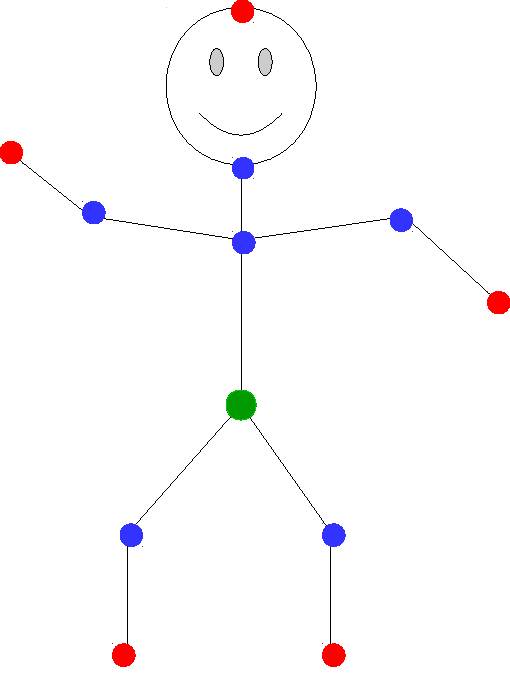
\includegraphics[height = 0.70\textwidth]{imagenes/palitos}
    \captionof{figure}{Cuerpo rígido de ejemplo. Nodo root en verde, nodos en azul y nodos terminales en rojo. A la derecha, ejemplo de como se describe la jerarquía.}
    \label{fig:palitos}
\end{minipage}
\begin{minipage}{0.5\textwidth}
    \begin{verbatim}
ROOT Cadera{
    JOINT PiernaDerecha{
        END PiernaDerecha{
        }
    }
    JOINT PiernaIzquierda{
        END PiernaIzquierda{
        }
    }
    JOINT Pecho{
        JOINT BrazoDerecho{
            END BrazoDerecho{
            }
        }
        JOINT BrazoIzquierdo{
            END Brazo Izquierdo{
            }
        }
        JOINT Cabeza{
            END Cabeza{
            }
        }
    }
}
    \end{verbatim}    
\end{minipage}

La figura \ref{code:joint} muestra la implementación de la estructura \mono{Joint} utilizada para \emph{parsear} la jerarquía de un archivo BVH. Al encontrar la palabra reservada \mono{ROOT}, \mono{JOINT} o \mono{END} se crea un nuevo Joint y se añade a un arreglo, excepto en el caso del ROOT, el puntero padre apunta al último Joint añadido al arreglo de padres. Al encontrar una llave izquierda \mono{\{} se toma el último Joint del arreglo Joints y se añade a un arreglo de padres, al encontrar una llave derecha \mono{\}} se elimina el último Joint del arreglo de padres. 

La siguiente sección explicará en detalle la función de las matices locales y globales, por ahora basta con decir que el valor de offset se almacena en la última columna de la matriz local. 

\begin{figure}
    \centering
    \begin{verbatim}
struct Joint{
    char * name;
    int isRoot;
    int isEnd;
    Joint * parent;
    double rotation[3];
    double * local_matrix;
    double * global_matrix;
}
    \end{verbatim}
    \caption{Implementación de la estructura \mono{Joint}}
    \label{code:joint}
\end{figure}

\section{MOTION}

Esta sección inicia con la palabra reservada \mono{MOTION}, a continuación se encuentran los valores \mono{Frames}, indica la cantidad de frames de la filmación y la palabra \mono{Frame time} que indica el periodo entre frames (el inverso de la frecuencia de grabación). Cada frame consiste en 6 valores en decimal para expresar el movimiento del nodo ROOT (3 para actualizar su posición global y 3 para su rotación) y 3 valores por cada Joint que no sea End. 

La matriz global y local de cada joint es una matriz $4 \times 4$, conformado por cuatro vectores columna, los primeros tres expresan rotación y siguiendo la convención en computación de graficos, tiene un cero en la cuarta fila. El cuarto vector columna expresa traslación y siguiendo la convención, tiene un uno en la cuarta fila, la ecuación \eqref{matriz_general} muestra esta convención.

\begin{equation}\label{matriz_general}
M = 
    \begin{pmatrix}
    r_{xx} & r_{xy} & r_{xz} & t_x \\
    r_{yx} & r_{yy} & r_{yz} & t_y \\
    r_{zx} & r_{zy} & r_{zz} & t_z \\
    0      & 0      & 0      & 1 
    \end{pmatrix}
\end{equation}

Los valores $t$ corresponden al offset encontrado en la sección \mono{HIERARCHY}, los valores $r$ Se obtiene la multiplicar las matrices de rotación $R_z$, $R_y$ y $R_x$, según explica \cite{andreas}, como se muestra en \eqref{matriz_rotacion}, los valores de los ángulos representados por $\theta$ en la ecuación son los valores que aparecen en esta sección, como se puede observar, son tres por Joint para formar la matriz. 

\begin{equation}\label{matriz_rotacion}
R_z R_y R_x = 
\begin{pmatrix}
 cos\ \theta_z & - sin\ \theta_z & 0 \\
 sin\ \theta_z & cos\ \theta_z & 0 \\
 0 & 0 & 1 
\end{pmatrix}
\begin{pmatrix}
 cos\ \theta_y & 0 & sin\ \theta_y \\
 0 & 1 & 0 \\
 - sin\ \theta_y & 0 & cos\ \theta_y 
\end{pmatrix}
\begin{pmatrix}
 1 & 0 & 0 \\
 0 & cos\ \theta_x & - sin\ \theta_x \\
 0 & sin\ \theta_x & cos\ \theta_x 
\end{pmatrix}
\end{equation}

En el caso de ROOT, la matriz global y local son la misma, pues el nodo ROOT existe en el marco de referencia global, para los demás nodos, se construye la matriz local, tal como se explicó anteriormente y se multiplica por la matriz global del nodo padre, claramente esta es una acción recursiva, pues se debe llegar hasta el nodo ROOT, como se muestra a continuación \eqref{matriz_recursiva}.

\begin{equation}\label{matriz_recursiva}
    M_{\text{global}} = M_{\text{local}} M_{\text{global\_padre}} M_{\text{global\_abuelo}} ... M_{\text{global\_root}}
\end{equation}

Finalmente, la posición de cada nodo respecto al marco de referencia global se encuentra en el cuarto vector columna de la matriz global. 
    El siguiente es un extracto de un archivo BVH con su primer frame.

\begin{verbatim}
HIERARCHY
ROOT Hips
{
  OFFSET 0.000000 0.000000 0.000000
  CHANNELS 6 Xposition Yposition Zposition Zrotation Xrotation Yrotation
  JOINT Spine
  {
    OFFSET -0.000000 0.076886 0.000000
    CHANNELS 3 Zrotation Xrotation Yrotation
    JOINT Spine1
    {
      OFFSET -0.000000 0.200136 0.000000
      CHANNELS 3 Zrotation Xrotation Yrotation
      JOINT Neck
      {
        OFFSET -0.000000 0.199314 0.018119
        CHANNELS 3 Zrotation Xrotation Yrotation
        JOINT Head
        {
          OFFSET -0.000000 0.131269 -0.018753
          CHANNELS 3 Zrotation Xrotation Yrotation
          End Site
          {
            OFFSET -0.000000 0.187528 0.000000
          }
        }
      }
      JOINT LeftShoulder
      {
        OFFSET 0.037527 0.175039 -0.003779
        CHANNELS 3 Zrotation Xrotation Yrotation
        JOINT LeftArm
        {
          OFFSET 0.133636 0.000000 0.000000
          CHANNELS 3 Zrotation Xrotation Yrotation
          JOINT LeftForeArm
          {
            OFFSET 0.299034 0.000000 0.000000
            CHANNELS 3 Zrotation Xrotation Yrotation
            JOINT LeftHand
            {
              OFFSET 0.221443 0.000000 0.000000
              CHANNELS 3 Zrotation Xrotation Yrotation
              End Site
              {
                OFFSET 0.140646 0.000000 0.000000
              }
            }
          }
        }
      }
      JOINT RightShoulder
      {
        OFFSET -0.037320 0.175039 -0.003779
        CHANNELS 3 Zrotation Xrotation Yrotation
        JOINT RightArm
        {
          OFFSET -0.133636 0.000000 0.000000
          CHANNELS 3 Zrotation Xrotation Yrotation
          JOINT RightForeArm
          {
            OFFSET -0.299034 0.000000 0.000000
            CHANNELS 3 Zrotation Xrotation Yrotation
            JOINT RightHand
            {
              OFFSET -0.221443 0.000000 0.000000
              CHANNELS 3 Zrotation Xrotation Yrotation
              End Site
              {
                OFFSET -0.140646 0.000000 0.000000
              }
            }
          }
        }
      }
    }
  }
  JOINT LeftUpLeg
  {
    OFFSET 0.093764 0.000000 0.000000
    CHANNELS 3 Zrotation Xrotation Yrotation
    JOINT LeftLeg
    {
      OFFSET -0.000000 -0.396379 0.000000
      CHANNELS 3 Zrotation Xrotation Yrotation
      JOINT LeftFoot
      {
        OFFSET -0.000000 -0.402188 0.000000
        CHANNELS 3 Zrotation Xrotation Yrotation
        JOINT LeftToeBase
        {
          OFFSET -0.000000 -0.060946 0.140646
          CHANNELS 3 Zrotation Xrotation Yrotation
          End Site
          {
            OFFSET -0.000000 0.000000 0.037506
          }
        }
      }
    }
  }
  JOINT RightUpLeg
  {
    OFFSET -0.093764 0.000000 0.000000
    CHANNELS 3 Zrotation Xrotation Yrotation
    JOINT RightLeg
    {
      OFFSET -0.000000 -0.396379 0.000000
      CHANNELS 3 Zrotation Xrotation Yrotation
      JOINT RightFoot
      {
        OFFSET -0.000000 -0.402188 0.000000
        CHANNELS 3 Zrotation Xrotation Yrotation
        JOINT RightToeBase
        {
          OFFSET -0.000000 -0.060946 0.140646
          CHANNELS 3 Zrotation Xrotation Yrotation
          End Site
          {
            OFFSET -0.000000 0.000000 0.037506
          }
        }
      }
    }
  }
}
MOTION
Frames:    19765
Frame Time:    0.003906
3.559094    0.923209    0.525318    0.013638    0.239340    -92.314423    -0.866819    
-8.201900   -1.085093    0.390321    1.095642    -0.341925    11.942478    19.273811
6.916184    -14.095366    1.028759    5.660420    16.413609    3.670976    6.878858
-20.665810  -4.967050    -7.953991    -9.244185    7.996674    -9.049491    -0.397082
7.268273    0.493494    -11.031128    2.884695    3.247415    18.525766    3.898051
3.358436    10.172389    6.814506    11.962240    1.635878    5.769930    1.235742
1.274122    6.534966    4.544692    -3.154521    -1.556152    -2.001814    1.299514
-4.085289    6.960749    0.023962    0.327613    -0.119950    -1.233113    4.604572
-3.182750    2.910497    5.662087    0.776524    -0.874389    -9.110942    -3.389380
-0.066035    -0.925920    0.191887    
\end{verbatim}

\chapter{Algoritmo de detección de los pasos}

El algoritmo presentado se inspira fuertemente en la idea presentada por \cite{scholkmann} llamado \emph{automatic multiscale-based peak detection} (AMPD). La intensión era generar un algoritmo de detección de picos para señales periódicas o cuasi-periódicas robusto al ruido de baja frecuencia y que no necesitara parámetros. La estructura principal del algoritmo es el \emph{local maxima scalogram} una matriz tamaño $N \times N/2$, donde N es el tamaño del vector de datos. Esta matriz se llena de la siguiente manera: se selecciona un tamaño de ventana $w = 2k | k = 1, 2, 3, ..., N/2$, esta ventana se desplaza por el vector de datos y si el valor en el centro de la ventana es el máximo, se almacena un cero, de otra manera se almacena un número aleatorio entre 1 y 2, tal como muestra \eqref{ampd_matriz}, donde $r$ es un número aleatorio entre 0 y 1.

\begin{equation}\label{ampd_matriz}
    w_{i,k} =
    \begin{cases}
    0\ , & \quad \text{si}\ i\ \text{es máximo} \\ 
    1 + r\ , & \quad \text{de otra manera} 
    \end{cases}
\end{equation}

Note que construir esta matriz es un algoritmo $O(N^2)$ y es la parte más lenta del algoritmo. Una vez construida se hace una suma por filas y como criterio para seleccionar el tamaño de ventana adecuado se toma la fila que suma menor valor, se descartan los valores de ventana mayores y se eliminan de la matriz. Después se calculará la desviación estándar por columna y en los casos donde esta resulte $0$ se encuentra un máximo. 

El criterio utilizado para seleccionar el valor óptimo de ventada tiene una consecuencia interesante: la frecuencia máxima de la señal no puede se mayor a 4 veces la frecuencia mínima de la señal $f_{max} < 4 f_{min}$, este no es el caso de la marcha, por lo tanto se propone otro algoritmo, semejante al AMPD.

\begin{figure}
    \centering
    % GNUPLOT: LaTeX picture
\setlength{\unitlength}{0.240900pt}
\ifx\plotpoint\undefined\newsavebox{\plotpoint}\fi
\begin{picture}(1500,900)(0,0)
\sbox{\plotpoint}{\rule[-0.200pt]{0.400pt}{0.400pt}}%
\put(191.0,131.0){\rule[-0.200pt]{4.818pt}{0.400pt}}
\put(171,131){\makebox(0,0)[r]{ 0.05}}
\put(1419.0,131.0){\rule[-0.200pt]{4.818pt}{0.400pt}}
\put(191.0,239.0){\rule[-0.200pt]{4.818pt}{0.400pt}}
\put(171,239){\makebox(0,0)[r]{ 0.1}}
\put(1419.0,239.0){\rule[-0.200pt]{4.818pt}{0.400pt}}
\put(191.0,346.0){\rule[-0.200pt]{4.818pt}{0.400pt}}
\put(171,346){\makebox(0,0)[r]{ 0.15}}
\put(1419.0,346.0){\rule[-0.200pt]{4.818pt}{0.400pt}}
\put(191.0,454.0){\rule[-0.200pt]{4.818pt}{0.400pt}}
\put(171,454){\makebox(0,0)[r]{ 0.2}}
\put(1419.0,454.0){\rule[-0.200pt]{4.818pt}{0.400pt}}
\put(191.0,561.0){\rule[-0.200pt]{4.818pt}{0.400pt}}
\put(171,561){\makebox(0,0)[r]{ 0.25}}
\put(1419.0,561.0){\rule[-0.200pt]{4.818pt}{0.400pt}}
\put(191.0,669.0){\rule[-0.200pt]{4.818pt}{0.400pt}}
\put(171,669){\makebox(0,0)[r]{ 0.3}}
\put(1419.0,669.0){\rule[-0.200pt]{4.818pt}{0.400pt}}
\put(191.0,776.0){\rule[-0.200pt]{4.818pt}{0.400pt}}
\put(171,776){\makebox(0,0)[r]{ 0.35}}
\put(1419.0,776.0){\rule[-0.200pt]{4.818pt}{0.400pt}}
\put(333.0,131.0){\rule[-0.200pt]{0.400pt}{4.818pt}}
\put(333,90){\makebox(0,0){ 400}}
\put(333.0,756.0){\rule[-0.200pt]{0.400pt}{4.818pt}}
\put(542.0,131.0){\rule[-0.200pt]{0.400pt}{4.818pt}}
\put(542,90){\makebox(0,0){ 600}}
\put(542.0,756.0){\rule[-0.200pt]{0.400pt}{4.818pt}}
\put(752.0,131.0){\rule[-0.200pt]{0.400pt}{4.818pt}}
\put(752,90){\makebox(0,0){ 800}}
\put(752.0,756.0){\rule[-0.200pt]{0.400pt}{4.818pt}}
\put(962.0,131.0){\rule[-0.200pt]{0.400pt}{4.818pt}}
\put(962,90){\makebox(0,0){ 1000}}
\put(962.0,756.0){\rule[-0.200pt]{0.400pt}{4.818pt}}
\put(1172.0,131.0){\rule[-0.200pt]{0.400pt}{4.818pt}}
\put(1172,90){\makebox(0,0){ 1200}}
\put(1172.0,756.0){\rule[-0.200pt]{0.400pt}{4.818pt}}
\put(1381.0,131.0){\rule[-0.200pt]{0.400pt}{4.818pt}}
\put(1381,90){\makebox(0,0){ 1400}}
\put(1381.0,756.0){\rule[-0.200pt]{0.400pt}{4.818pt}}
\put(191.0,131.0){\rule[-0.200pt]{0.400pt}{155.380pt}}
\put(191.0,131.0){\rule[-0.200pt]{300.643pt}{0.400pt}}
\put(1439.0,131.0){\rule[-0.200pt]{0.400pt}{155.380pt}}
\put(191.0,776.0){\rule[-0.200pt]{300.643pt}{0.400pt}}
\put(30,453){\makebox(0,0){\rotatebox{90}{Altura (m)}}}
\put(815,29){\makebox(0,0){Frames}}
\put(815,838){\makebox(0,0){Altura del talon}}
\put(191,237){\rule{1pt}{1pt}}
\put(192,237){\rule{1pt}{1pt}}
\put(193,236){\rule{1pt}{1pt}}
\put(194,236){\rule{1pt}{1pt}}
\put(195,235){\rule{1pt}{1pt}}
\put(196,234){\rule{1pt}{1pt}}
\put(197,234){\rule{1pt}{1pt}}
\put(198,233){\rule{1pt}{1pt}}
\put(199,233){\rule{1pt}{1pt}}
\put(200,233){\rule{1pt}{1pt}}
\put(201,233){\rule{1pt}{1pt}}
\put(203,233){\rule{1pt}{1pt}}
\put(204,233){\rule{1pt}{1pt}}
\put(205,234){\rule{1pt}{1pt}}
\put(206,234){\rule{1pt}{1pt}}
\put(207,234){\rule{1pt}{1pt}}
\put(208,235){\rule{1pt}{1pt}}
\put(209,235){\rule{1pt}{1pt}}
\put(210,235){\rule{1pt}{1pt}}
\put(211,236){\rule{1pt}{1pt}}
\put(212,236){\rule{1pt}{1pt}}
\put(213,237){\rule{1pt}{1pt}}
\put(214,237){\rule{1pt}{1pt}}
\put(215,238){\rule{1pt}{1pt}}
\put(216,238){\rule{1pt}{1pt}}
\put(217,239){\rule{1pt}{1pt}}
\put(218,239){\rule{1pt}{1pt}}
\put(219,240){\rule{1pt}{1pt}}
\put(220,240){\rule{1pt}{1pt}}
\put(221,241){\rule{1pt}{1pt}}
\put(222,241){\rule{1pt}{1pt}}
\put(224,242){\rule{1pt}{1pt}}
\put(225,241){\rule{1pt}{1pt}}
\put(226,242){\rule{1pt}{1pt}}
\put(227,242){\rule{1pt}{1pt}}
\put(228,242){\rule{1pt}{1pt}}
\put(229,242){\rule{1pt}{1pt}}
\put(230,242){\rule{1pt}{1pt}}
\put(231,243){\rule{1pt}{1pt}}
\put(232,243){\rule{1pt}{1pt}}
\put(233,243){\rule{1pt}{1pt}}
\put(234,242){\rule{1pt}{1pt}}
\put(235,243){\rule{1pt}{1pt}}
\put(236,243){\rule{1pt}{1pt}}
\put(237,244){\rule{1pt}{1pt}}
\put(238,244){\rule{1pt}{1pt}}
\put(239,244){\rule{1pt}{1pt}}
\put(240,244){\rule{1pt}{1pt}}
\put(241,244){\rule{1pt}{1pt}}
\put(242,245){\rule{1pt}{1pt}}
\put(243,245){\rule{1pt}{1pt}}
\put(244,246){\rule{1pt}{1pt}}
\put(246,247){\rule{1pt}{1pt}}
\put(247,245){\rule{1pt}{1pt}}
\put(248,247){\rule{1pt}{1pt}}
\put(249,249){\rule{1pt}{1pt}}
\put(250,248){\rule{1pt}{1pt}}
\put(251,251){\rule{1pt}{1pt}}
\put(252,248){\rule{1pt}{1pt}}
\put(253,249){\rule{1pt}{1pt}}
\put(254,249){\rule{1pt}{1pt}}
\put(255,244){\rule{1pt}{1pt}}
\put(256,250){\rule{1pt}{1pt}}
\put(257,250){\rule{1pt}{1pt}}
\put(258,248){\rule{1pt}{1pt}}
\put(259,249){\rule{1pt}{1pt}}
\put(260,249){\rule{1pt}{1pt}}
\put(261,256){\rule{1pt}{1pt}}
\put(262,253){\rule{1pt}{1pt}}
\put(263,249){\rule{1pt}{1pt}}
\put(264,252){\rule{1pt}{1pt}}
\put(265,252){\rule{1pt}{1pt}}
\put(267,253){\rule{1pt}{1pt}}
\put(268,253){\rule{1pt}{1pt}}
\put(269,254){\rule{1pt}{1pt}}
\put(270,255){\rule{1pt}{1pt}}
\put(271,257){\rule{1pt}{1pt}}
\put(272,258){\rule{1pt}{1pt}}
\put(273,259){\rule{1pt}{1pt}}
\put(274,260){\rule{1pt}{1pt}}
\put(275,262){\rule{1pt}{1pt}}
\put(276,264){\rule{1pt}{1pt}}
\put(277,266){\rule{1pt}{1pt}}
\put(278,268){\rule{1pt}{1pt}}
\put(279,270){\rule{1pt}{1pt}}
\put(280,273){\rule{1pt}{1pt}}
\put(281,276){\rule{1pt}{1pt}}
\put(282,278){\rule{1pt}{1pt}}
\put(283,281){\rule{1pt}{1pt}}
\put(284,285){\rule{1pt}{1pt}}
\put(285,288){\rule{1pt}{1pt}}
\put(286,292){\rule{1pt}{1pt}}
\put(287,296){\rule{1pt}{1pt}}
\put(289,300){\rule{1pt}{1pt}}
\put(290,304){\rule{1pt}{1pt}}
\put(291,308){\rule{1pt}{1pt}}
\put(292,313){\rule{1pt}{1pt}}
\put(293,318){\rule{1pt}{1pt}}
\put(294,324){\rule{1pt}{1pt}}
\put(295,329){\rule{1pt}{1pt}}
\put(296,335){\rule{1pt}{1pt}}
\put(297,341){\rule{1pt}{1pt}}
\put(298,347){\rule{1pt}{1pt}}
\put(299,353){\rule{1pt}{1pt}}
\put(300,359){\rule{1pt}{1pt}}
\put(301,365){\rule{1pt}{1pt}}
\put(302,372){\rule{1pt}{1pt}}
\put(303,379){\rule{1pt}{1pt}}
\put(304,385){\rule{1pt}{1pt}}
\put(305,392){\rule{1pt}{1pt}}
\put(306,399){\rule{1pt}{1pt}}
\put(307,406){\rule{1pt}{1pt}}
\put(308,413){\rule{1pt}{1pt}}
\put(310,420){\rule{1pt}{1pt}}
\put(311,427){\rule{1pt}{1pt}}
\put(312,434){\rule{1pt}{1pt}}
\put(313,442){\rule{1pt}{1pt}}
\put(314,449){\rule{1pt}{1pt}}
\put(315,457){\rule{1pt}{1pt}}
\put(316,465){\rule{1pt}{1pt}}
\put(317,473){\rule{1pt}{1pt}}
\put(318,481){\rule{1pt}{1pt}}
\put(319,490){\rule{1pt}{1pt}}
\put(320,499){\rule{1pt}{1pt}}
\put(321,508){\rule{1pt}{1pt}}
\put(322,517){\rule{1pt}{1pt}}
\put(323,525){\rule{1pt}{1pt}}
\put(324,533){\rule{1pt}{1pt}}
\put(325,541){\rule{1pt}{1pt}}
\put(326,551){\rule{1pt}{1pt}}
\put(327,560){\rule{1pt}{1pt}}
\put(328,568){\rule{1pt}{1pt}}
\put(329,575){\rule{1pt}{1pt}}
\put(330,583){\rule{1pt}{1pt}}
\put(332,590){\rule{1pt}{1pt}}
\put(333,596){\rule{1pt}{1pt}}
\put(334,602){\rule{1pt}{1pt}}
\put(335,608){\rule{1pt}{1pt}}
\put(336,612){\rule{1pt}{1pt}}
\put(337,615){\rule{1pt}{1pt}}
\put(338,618){\rule{1pt}{1pt}}
\put(339,619){\rule{1pt}{1pt}}
\put(340,620){\rule{1pt}{1pt}}
\put(341,620){\rule{1pt}{1pt}}
\put(342,619){\rule{1pt}{1pt}}
\put(343,618){\rule{1pt}{1pt}}
\put(344,616){\rule{1pt}{1pt}}
\put(345,613){\rule{1pt}{1pt}}
\put(346,610){\rule{1pt}{1pt}}
\put(347,606){\rule{1pt}{1pt}}
\put(348,601){\rule{1pt}{1pt}}
\put(349,596){\rule{1pt}{1pt}}
\put(350,589){\rule{1pt}{1pt}}
\put(351,583){\rule{1pt}{1pt}}
\put(353,576){\rule{1pt}{1pt}}
\put(354,569){\rule{1pt}{1pt}}
\put(355,561){\rule{1pt}{1pt}}
\put(356,553){\rule{1pt}{1pt}}
\put(357,545){\rule{1pt}{1pt}}
\put(358,536){\rule{1pt}{1pt}}
\put(359,528){\rule{1pt}{1pt}}
\put(360,519){\rule{1pt}{1pt}}
\put(361,511){\rule{1pt}{1pt}}
\put(362,502){\rule{1pt}{1pt}}
\put(363,493){\rule{1pt}{1pt}}
\put(364,484){\rule{1pt}{1pt}}
\put(365,474){\rule{1pt}{1pt}}
\put(366,464){\rule{1pt}{1pt}}
\put(367,455){\rule{1pt}{1pt}}
\put(368,446){\rule{1pt}{1pt}}
\put(369,436){\rule{1pt}{1pt}}
\put(370,427){\rule{1pt}{1pt}}
\put(371,418){\rule{1pt}{1pt}}
\put(372,409){\rule{1pt}{1pt}}
\put(373,401){\rule{1pt}{1pt}}
\put(375,392){\rule{1pt}{1pt}}
\put(376,384){\rule{1pt}{1pt}}
\put(377,376){\rule{1pt}{1pt}}
\put(378,368){\rule{1pt}{1pt}}
\put(379,360){\rule{1pt}{1pt}}
\put(380,352){\rule{1pt}{1pt}}
\put(381,345){\rule{1pt}{1pt}}
\put(382,339){\rule{1pt}{1pt}}
\put(383,332){\rule{1pt}{1pt}}
\put(384,325){\rule{1pt}{1pt}}
\put(385,319){\rule{1pt}{1pt}}
\put(386,313){\rule{1pt}{1pt}}
\put(387,308){\rule{1pt}{1pt}}
\put(388,303){\rule{1pt}{1pt}}
\put(389,299){\rule{1pt}{1pt}}
\put(390,294){\rule{1pt}{1pt}}
\put(391,290){\rule{1pt}{1pt}}
\put(392,287){\rule{1pt}{1pt}}
\put(393,284){\rule{1pt}{1pt}}
\put(394,281){\rule{1pt}{1pt}}
\put(396,279){\rule{1pt}{1pt}}
\put(397,277){\rule{1pt}{1pt}}
\put(398,275){\rule{1pt}{1pt}}
\put(399,273){\rule{1pt}{1pt}}
\put(400,273){\rule{1pt}{1pt}}
\put(401,272){\rule{1pt}{1pt}}
\put(402,272){\rule{1pt}{1pt}}
\put(403,272){\rule{1pt}{1pt}}
\put(404,272){\rule{1pt}{1pt}}
\put(405,273){\rule{1pt}{1pt}}
\put(406,274){\rule{1pt}{1pt}}
\put(407,275){\rule{1pt}{1pt}}
\put(408,277){\rule{1pt}{1pt}}
\put(409,278){\rule{1pt}{1pt}}
\put(410,280){\rule{1pt}{1pt}}
\put(411,282){\rule{1pt}{1pt}}
\put(412,284){\rule{1pt}{1pt}}
\put(413,286){\rule{1pt}{1pt}}
\put(414,288){\rule{1pt}{1pt}}
\put(415,289){\rule{1pt}{1pt}}
\put(416,291){\rule{1pt}{1pt}}
\put(418,292){\rule{1pt}{1pt}}
\put(419,293){\rule{1pt}{1pt}}
\put(420,294){\rule{1pt}{1pt}}
\put(421,294){\rule{1pt}{1pt}}
\put(422,293){\rule{1pt}{1pt}}
\put(423,293){\rule{1pt}{1pt}}
\put(424,291){\rule{1pt}{1pt}}
\put(425,290){\rule{1pt}{1pt}}
\put(426,288){\rule{1pt}{1pt}}
\put(427,285){\rule{1pt}{1pt}}
\put(428,282){\rule{1pt}{1pt}}
\put(429,279){\rule{1pt}{1pt}}
\put(430,276){\rule{1pt}{1pt}}
\put(431,272){\rule{1pt}{1pt}}
\put(432,268){\rule{1pt}{1pt}}
\put(433,264){\rule{1pt}{1pt}}
\put(434,260){\rule{1pt}{1pt}}
\put(435,255){\rule{1pt}{1pt}}
\put(436,251){\rule{1pt}{1pt}}
\put(437,248){\rule{1pt}{1pt}}
\put(439,245){\rule{1pt}{1pt}}
\put(440,242){\rule{1pt}{1pt}}
\put(441,240){\rule{1pt}{1pt}}
\put(442,237){\rule{1pt}{1pt}}
\put(443,235){\rule{1pt}{1pt}}
\put(444,232){\rule{1pt}{1pt}}
\put(445,231){\rule{1pt}{1pt}}
\put(446,229){\rule{1pt}{1pt}}
\put(447,227){\rule{1pt}{1pt}}
\put(448,226){\rule{1pt}{1pt}}
\put(449,225){\rule{1pt}{1pt}}
\put(450,224){\rule{1pt}{1pt}}
\put(451,223){\rule{1pt}{1pt}}
\put(452,222){\rule{1pt}{1pt}}
\put(453,222){\rule{1pt}{1pt}}
\put(454,222){\rule{1pt}{1pt}}
\put(455,222){\rule{1pt}{1pt}}
\put(456,222){\rule{1pt}{1pt}}
\put(457,222){\rule{1pt}{1pt}}
\put(458,222){\rule{1pt}{1pt}}
\put(459,222){\rule{1pt}{1pt}}
\put(461,222){\rule{1pt}{1pt}}
\put(462,222){\rule{1pt}{1pt}}
\put(463,222){\rule{1pt}{1pt}}
\put(464,222){\rule{1pt}{1pt}}
\put(465,222){\rule{1pt}{1pt}}
\put(466,222){\rule{1pt}{1pt}}
\put(467,222){\rule{1pt}{1pt}}
\put(468,222){\rule{1pt}{1pt}}
\put(469,222){\rule{1pt}{1pt}}
\put(470,221){\rule{1pt}{1pt}}
\put(471,221){\rule{1pt}{1pt}}
\put(472,221){\rule{1pt}{1pt}}
\put(473,222){\rule{1pt}{1pt}}
\put(474,221){\rule{1pt}{1pt}}
\put(475,222){\rule{1pt}{1pt}}
\put(476,222){\rule{1pt}{1pt}}
\put(477,222){\rule{1pt}{1pt}}
\put(478,223){\rule{1pt}{1pt}}
\put(479,223){\rule{1pt}{1pt}}
\put(480,224){\rule{1pt}{1pt}}
\put(482,224){\rule{1pt}{1pt}}
\put(483,225){\rule{1pt}{1pt}}
\put(484,226){\rule{1pt}{1pt}}
\put(485,227){\rule{1pt}{1pt}}
\put(486,227){\rule{1pt}{1pt}}
\put(487,228){\rule{1pt}{1pt}}
\put(488,229){\rule{1pt}{1pt}}
\put(489,230){\rule{1pt}{1pt}}
\put(490,231){\rule{1pt}{1pt}}
\put(491,232){\rule{1pt}{1pt}}
\put(492,233){\rule{1pt}{1pt}}
\put(493,234){\rule{1pt}{1pt}}
\put(494,234){\rule{1pt}{1pt}}
\put(495,235){\rule{1pt}{1pt}}
\put(496,236){\rule{1pt}{1pt}}
\put(497,237){\rule{1pt}{1pt}}
\put(498,238){\rule{1pt}{1pt}}
\put(499,239){\rule{1pt}{1pt}}
\put(500,239){\rule{1pt}{1pt}}
\put(501,240){\rule{1pt}{1pt}}
\put(502,241){\rule{1pt}{1pt}}
\put(504,241){\rule{1pt}{1pt}}
\put(505,242){\rule{1pt}{1pt}}
\put(506,243){\rule{1pt}{1pt}}
\put(507,243){\rule{1pt}{1pt}}
\put(508,244){\rule{1pt}{1pt}}
\put(509,245){\rule{1pt}{1pt}}
\put(510,245){\rule{1pt}{1pt}}
\put(511,246){\rule{1pt}{1pt}}
\put(512,247){\rule{1pt}{1pt}}
\put(513,247){\rule{1pt}{1pt}}
\put(514,248){\rule{1pt}{1pt}}
\put(515,248){\rule{1pt}{1pt}}
\put(516,249){\rule{1pt}{1pt}}
\put(517,249){\rule{1pt}{1pt}}
\put(518,250){\rule{1pt}{1pt}}
\put(519,250){\rule{1pt}{1pt}}
\put(520,251){\rule{1pt}{1pt}}
\put(521,251){\rule{1pt}{1pt}}
\put(522,252){\rule{1pt}{1pt}}
\put(523,252){\rule{1pt}{1pt}}
\put(524,253){\rule{1pt}{1pt}}
\put(526,253){\rule{1pt}{1pt}}
\put(527,253){\rule{1pt}{1pt}}
\put(528,254){\rule{1pt}{1pt}}
\put(529,255){\rule{1pt}{1pt}}
\put(530,255){\rule{1pt}{1pt}}
\put(531,256){\rule{1pt}{1pt}}
\put(532,257){\rule{1pt}{1pt}}
\put(533,257){\rule{1pt}{1pt}}
\put(534,258){\rule{1pt}{1pt}}
\put(535,259){\rule{1pt}{1pt}}
\put(536,261){\rule{1pt}{1pt}}
\put(537,262){\rule{1pt}{1pt}}
\put(538,264){\rule{1pt}{1pt}}
\put(539,265){\rule{1pt}{1pt}}
\put(540,268){\rule{1pt}{1pt}}
\put(541,270){\rule{1pt}{1pt}}
\put(542,273){\rule{1pt}{1pt}}
\put(543,276){\rule{1pt}{1pt}}
\put(544,279){\rule{1pt}{1pt}}
\put(545,282){\rule{1pt}{1pt}}
\put(547,286){\rule{1pt}{1pt}}
\put(548,290){\rule{1pt}{1pt}}
\put(549,295){\rule{1pt}{1pt}}
\put(550,299){\rule{1pt}{1pt}}
\put(551,305){\rule{1pt}{1pt}}
\put(552,310){\rule{1pt}{1pt}}
\put(553,316){\rule{1pt}{1pt}}
\put(554,322){\rule{1pt}{1pt}}
\put(555,328){\rule{1pt}{1pt}}
\put(556,334){\rule{1pt}{1pt}}
\put(557,341){\rule{1pt}{1pt}}
\put(558,348){\rule{1pt}{1pt}}
\put(559,355){\rule{1pt}{1pt}}
\put(560,362){\rule{1pt}{1pt}}
\put(561,369){\rule{1pt}{1pt}}
\put(562,377){\rule{1pt}{1pt}}
\put(563,384){\rule{1pt}{1pt}}
\put(564,392){\rule{1pt}{1pt}}
\put(565,400){\rule{1pt}{1pt}}
\put(566,408){\rule{1pt}{1pt}}
\put(567,416){\rule{1pt}{1pt}}
\put(569,424){\rule{1pt}{1pt}}
\put(570,432){\rule{1pt}{1pt}}
\put(571,440){\rule{1pt}{1pt}}
\put(572,448){\rule{1pt}{1pt}}
\put(573,456){\rule{1pt}{1pt}}
\put(574,464){\rule{1pt}{1pt}}
\put(575,473){\rule{1pt}{1pt}}
\put(576,481){\rule{1pt}{1pt}}
\put(577,490){\rule{1pt}{1pt}}
\put(578,500){\rule{1pt}{1pt}}
\put(579,510){\rule{1pt}{1pt}}
\put(580,520){\rule{1pt}{1pt}}
\put(581,530){\rule{1pt}{1pt}}
\put(582,540){\rule{1pt}{1pt}}
\put(583,548){\rule{1pt}{1pt}}
\put(584,558){\rule{1pt}{1pt}}
\put(585,568){\rule{1pt}{1pt}}
\put(586,577){\rule{1pt}{1pt}}
\put(587,586){\rule{1pt}{1pt}}
\put(588,595){\rule{1pt}{1pt}}
\put(590,604){\rule{1pt}{1pt}}
\put(591,613){\rule{1pt}{1pt}}
\put(592,622){\rule{1pt}{1pt}}
\put(593,630){\rule{1pt}{1pt}}
\put(594,638){\rule{1pt}{1pt}}
\put(595,645){\rule{1pt}{1pt}}
\put(596,651){\rule{1pt}{1pt}}
\put(597,656){\rule{1pt}{1pt}}
\put(598,660){\rule{1pt}{1pt}}
\put(599,664){\rule{1pt}{1pt}}
\put(600,667){\rule{1pt}{1pt}}
\put(601,669){\rule{1pt}{1pt}}
\put(602,670){\rule{1pt}{1pt}}
\put(603,671){\rule{1pt}{1pt}}
\put(604,671){\rule{1pt}{1pt}}
\put(605,670){\rule{1pt}{1pt}}
\put(606,669){\rule{1pt}{1pt}}
\put(607,667){\rule{1pt}{1pt}}
\put(608,665){\rule{1pt}{1pt}}
\put(609,661){\rule{1pt}{1pt}}
\put(610,657){\rule{1pt}{1pt}}
\put(612,653){\rule{1pt}{1pt}}
\put(613,648){\rule{1pt}{1pt}}
\put(614,643){\rule{1pt}{1pt}}
\put(615,637){\rule{1pt}{1pt}}
\put(616,630){\rule{1pt}{1pt}}
\put(617,623){\rule{1pt}{1pt}}
\put(618,616){\rule{1pt}{1pt}}
\put(619,608){\rule{1pt}{1pt}}
\put(620,599){\rule{1pt}{1pt}}
\put(621,591){\rule{1pt}{1pt}}
\put(622,581){\rule{1pt}{1pt}}
\put(623,572){\rule{1pt}{1pt}}
\put(624,563){\rule{1pt}{1pt}}
\put(625,554){\rule{1pt}{1pt}}
\put(626,544){\rule{1pt}{1pt}}
\put(627,534){\rule{1pt}{1pt}}
\put(628,525){\rule{1pt}{1pt}}
\put(629,515){\rule{1pt}{1pt}}
\put(630,505){\rule{1pt}{1pt}}
\put(631,495){\rule{1pt}{1pt}}
\put(633,485){\rule{1pt}{1pt}}
\put(634,474){\rule{1pt}{1pt}}
\put(635,464){\rule{1pt}{1pt}}
\put(636,454){\rule{1pt}{1pt}}
\put(637,443){\rule{1pt}{1pt}}
\put(638,433){\rule{1pt}{1pt}}
\put(639,423){\rule{1pt}{1pt}}
\put(640,413){\rule{1pt}{1pt}}
\put(641,403){\rule{1pt}{1pt}}
\put(642,394){\rule{1pt}{1pt}}
\put(643,384){\rule{1pt}{1pt}}
\put(644,375){\rule{1pt}{1pt}}
\put(645,366){\rule{1pt}{1pt}}
\put(646,357){\rule{1pt}{1pt}}
\put(647,348){\rule{1pt}{1pt}}
\put(648,340){\rule{1pt}{1pt}}
\put(649,331){\rule{1pt}{1pt}}
\put(650,324){\rule{1pt}{1pt}}
\put(651,317){\rule{1pt}{1pt}}
\put(652,310){\rule{1pt}{1pt}}
\put(653,304){\rule{1pt}{1pt}}
\put(655,297){\rule{1pt}{1pt}}
\put(656,292){\rule{1pt}{1pt}}
\put(657,287){\rule{1pt}{1pt}}
\put(658,282){\rule{1pt}{1pt}}
\put(659,279){\rule{1pt}{1pt}}
\put(660,276){\rule{1pt}{1pt}}
\put(661,273){\rule{1pt}{1pt}}
\put(662,271){\rule{1pt}{1pt}}
\put(663,269){\rule{1pt}{1pt}}
\put(664,268){\rule{1pt}{1pt}}
\put(665,268){\rule{1pt}{1pt}}
\put(666,268){\rule{1pt}{1pt}}
\put(667,269){\rule{1pt}{1pt}}
\put(668,270){\rule{1pt}{1pt}}
\put(669,272){\rule{1pt}{1pt}}
\put(670,274){\rule{1pt}{1pt}}
\put(671,276){\rule{1pt}{1pt}}
\put(672,279){\rule{1pt}{1pt}}
\put(673,282){\rule{1pt}{1pt}}
\put(674,285){\rule{1pt}{1pt}}
\put(676,287){\rule{1pt}{1pt}}
\put(677,290){\rule{1pt}{1pt}}
\put(678,292){\rule{1pt}{1pt}}
\put(679,294){\rule{1pt}{1pt}}
\put(680,295){\rule{1pt}{1pt}}
\put(681,295){\rule{1pt}{1pt}}
\put(682,294){\rule{1pt}{1pt}}
\put(683,293){\rule{1pt}{1pt}}
\put(684,291){\rule{1pt}{1pt}}
\put(685,288){\rule{1pt}{1pt}}
\put(686,284){\rule{1pt}{1pt}}
\put(687,280){\rule{1pt}{1pt}}
\put(688,276){\rule{1pt}{1pt}}
\put(689,271){\rule{1pt}{1pt}}
\put(690,266){\rule{1pt}{1pt}}
\put(691,261){\rule{1pt}{1pt}}
\put(692,256){\rule{1pt}{1pt}}
\put(693,251){\rule{1pt}{1pt}}
\put(694,245){\rule{1pt}{1pt}}
\put(695,241){\rule{1pt}{1pt}}
\put(696,236){\rule{1pt}{1pt}}
\put(698,233){\rule{1pt}{1pt}}
\put(699,229){\rule{1pt}{1pt}}
\put(700,227){\rule{1pt}{1pt}}
\put(701,224){\rule{1pt}{1pt}}
\put(702,220){\rule{1pt}{1pt}}
\put(703,217){\rule{1pt}{1pt}}
\put(704,214){\rule{1pt}{1pt}}
\put(705,213){\rule{1pt}{1pt}}
\put(706,211){\rule{1pt}{1pt}}
\put(707,209){\rule{1pt}{1pt}}
\put(708,208){\rule{1pt}{1pt}}
\put(709,209){\rule{1pt}{1pt}}
\put(710,209){\rule{1pt}{1pt}}
\put(711,209){\rule{1pt}{1pt}}
\put(712,209){\rule{1pt}{1pt}}
\put(713,210){\rule{1pt}{1pt}}
\put(714,210){\rule{1pt}{1pt}}
\put(715,210){\rule{1pt}{1pt}}
\put(716,210){\rule{1pt}{1pt}}
\put(717,210){\rule{1pt}{1pt}}
\put(719,210){\rule{1pt}{1pt}}
\put(720,210){\rule{1pt}{1pt}}
\put(721,210){\rule{1pt}{1pt}}
\put(722,209){\rule{1pt}{1pt}}
\put(723,209){\rule{1pt}{1pt}}
\put(724,209){\rule{1pt}{1pt}}
\put(725,209){\rule{1pt}{1pt}}
\put(726,209){\rule{1pt}{1pt}}
\put(727,209){\rule{1pt}{1pt}}
\put(728,209){\rule{1pt}{1pt}}
\put(729,209){\rule{1pt}{1pt}}
\put(730,209){\rule{1pt}{1pt}}
\put(731,210){\rule{1pt}{1pt}}
\put(732,210){\rule{1pt}{1pt}}
\put(733,211){\rule{1pt}{1pt}}
\put(734,211){\rule{1pt}{1pt}}
\put(735,212){\rule{1pt}{1pt}}
\put(736,213){\rule{1pt}{1pt}}
\put(737,213){\rule{1pt}{1pt}}
\put(738,214){\rule{1pt}{1pt}}
\put(739,215){\rule{1pt}{1pt}}
\put(741,216){\rule{1pt}{1pt}}
\put(742,216){\rule{1pt}{1pt}}
\put(743,217){\rule{1pt}{1pt}}
\put(744,217){\rule{1pt}{1pt}}
\put(745,218){\rule{1pt}{1pt}}
\put(746,219){\rule{1pt}{1pt}}
\put(747,220){\rule{1pt}{1pt}}
\put(748,221){\rule{1pt}{1pt}}
\put(749,222){\rule{1pt}{1pt}}
\put(750,223){\rule{1pt}{1pt}}
\put(751,224){\rule{1pt}{1pt}}
\put(752,226){\rule{1pt}{1pt}}
\put(753,227){\rule{1pt}{1pt}}
\put(754,228){\rule{1pt}{1pt}}
\put(755,229){\rule{1pt}{1pt}}
\put(756,230){\rule{1pt}{1pt}}
\put(757,231){\rule{1pt}{1pt}}
\put(758,232){\rule{1pt}{1pt}}
\put(759,233){\rule{1pt}{1pt}}
\put(760,234){\rule{1pt}{1pt}}
\put(762,236){\rule{1pt}{1pt}}
\put(763,237){\rule{1pt}{1pt}}
\put(764,238){\rule{1pt}{1pt}}
\put(765,239){\rule{1pt}{1pt}}
\put(766,240){\rule{1pt}{1pt}}
\put(767,241){\rule{1pt}{1pt}}
\put(768,242){\rule{1pt}{1pt}}
\put(769,243){\rule{1pt}{1pt}}
\put(770,244){\rule{1pt}{1pt}}
\put(771,244){\rule{1pt}{1pt}}
\put(772,245){\rule{1pt}{1pt}}
\put(773,246){\rule{1pt}{1pt}}
\put(774,247){\rule{1pt}{1pt}}
\put(775,247){\rule{1pt}{1pt}}
\put(776,248){\rule{1pt}{1pt}}
\put(777,248){\rule{1pt}{1pt}}
\put(778,249){\rule{1pt}{1pt}}
\put(779,249){\rule{1pt}{1pt}}
\put(780,250){\rule{1pt}{1pt}}
\put(781,250){\rule{1pt}{1pt}}
\put(782,251){\rule{1pt}{1pt}}
\put(784,252){\rule{1pt}{1pt}}
\put(785,252){\rule{1pt}{1pt}}
\put(786,253){\rule{1pt}{1pt}}
\put(787,253){\rule{1pt}{1pt}}
\put(788,254){\rule{1pt}{1pt}}
\put(789,255){\rule{1pt}{1pt}}
\put(790,256){\rule{1pt}{1pt}}
\put(791,257){\rule{1pt}{1pt}}
\put(792,259){\rule{1pt}{1pt}}
\put(793,260){\rule{1pt}{1pt}}
\put(794,262){\rule{1pt}{1pt}}
\put(795,264){\rule{1pt}{1pt}}
\put(796,266){\rule{1pt}{1pt}}
\put(797,268){\rule{1pt}{1pt}}
\put(798,270){\rule{1pt}{1pt}}
\put(799,273){\rule{1pt}{1pt}}
\put(800,276){\rule{1pt}{1pt}}
\put(801,279){\rule{1pt}{1pt}}
\put(802,283){\rule{1pt}{1pt}}
\put(803,286){\rule{1pt}{1pt}}
\put(805,291){\rule{1pt}{1pt}}
\put(806,296){\rule{1pt}{1pt}}
\put(807,300){\rule{1pt}{1pt}}
\put(808,306){\rule{1pt}{1pt}}
\put(809,311){\rule{1pt}{1pt}}
\put(810,317){\rule{1pt}{1pt}}
\put(811,323){\rule{1pt}{1pt}}
\put(812,329){\rule{1pt}{1pt}}
\put(813,335){\rule{1pt}{1pt}}
\put(814,342){\rule{1pt}{1pt}}
\put(815,349){\rule{1pt}{1pt}}
\put(816,356){\rule{1pt}{1pt}}
\put(817,364){\rule{1pt}{1pt}}
\put(818,372){\rule{1pt}{1pt}}
\put(819,379){\rule{1pt}{1pt}}
\put(820,387){\rule{1pt}{1pt}}
\put(821,395){\rule{1pt}{1pt}}
\put(822,403){\rule{1pt}{1pt}}
\put(823,410){\rule{1pt}{1pt}}
\put(824,418){\rule{1pt}{1pt}}
\put(825,426){\rule{1pt}{1pt}}
\put(827,434){\rule{1pt}{1pt}}
\put(828,442){\rule{1pt}{1pt}}
\put(829,450){\rule{1pt}{1pt}}
\put(830,458){\rule{1pt}{1pt}}
\put(831,466){\rule{1pt}{1pt}}
\put(832,475){\rule{1pt}{1pt}}
\put(833,484){\rule{1pt}{1pt}}
\put(834,492){\rule{1pt}{1pt}}
\put(835,501){\rule{1pt}{1pt}}
\put(836,510){\rule{1pt}{1pt}}
\put(837,519){\rule{1pt}{1pt}}
\put(838,527){\rule{1pt}{1pt}}
\put(839,535){\rule{1pt}{1pt}}
\put(840,546){\rule{1pt}{1pt}}
\put(841,554){\rule{1pt}{1pt}}
\put(842,563){\rule{1pt}{1pt}}
\put(843,571){\rule{1pt}{1pt}}
\put(844,579){\rule{1pt}{1pt}}
\put(845,586){\rule{1pt}{1pt}}
\put(846,594){\rule{1pt}{1pt}}
\put(848,602){\rule{1pt}{1pt}}
\put(849,609){\rule{1pt}{1pt}}
\put(850,615){\rule{1pt}{1pt}}
\put(851,621){\rule{1pt}{1pt}}
\put(852,626){\rule{1pt}{1pt}}
\put(853,630){\rule{1pt}{1pt}}
\put(854,633){\rule{1pt}{1pt}}
\put(855,636){\rule{1pt}{1pt}}
\put(856,638){\rule{1pt}{1pt}}
\put(857,639){\rule{1pt}{1pt}}
\put(858,640){\rule{1pt}{1pt}}
\put(859,640){\rule{1pt}{1pt}}
\put(860,640){\rule{1pt}{1pt}}
\put(861,639){\rule{1pt}{1pt}}
\put(862,637){\rule{1pt}{1pt}}
\put(863,635){\rule{1pt}{1pt}}
\put(864,631){\rule{1pt}{1pt}}
\put(865,628){\rule{1pt}{1pt}}
\put(866,623){\rule{1pt}{1pt}}
\put(867,619){\rule{1pt}{1pt}}
\put(868,613){\rule{1pt}{1pt}}
\put(870,608){\rule{1pt}{1pt}}
\put(871,602){\rule{1pt}{1pt}}
\put(872,595){\rule{1pt}{1pt}}
\put(873,588){\rule{1pt}{1pt}}
\put(874,580){\rule{1pt}{1pt}}
\put(875,573){\rule{1pt}{1pt}}
\put(876,564){\rule{1pt}{1pt}}
\put(877,556){\rule{1pt}{1pt}}
\put(878,546){\rule{1pt}{1pt}}
\put(879,537){\rule{1pt}{1pt}}
\put(880,529){\rule{1pt}{1pt}}
\put(881,519){\rule{1pt}{1pt}}
\put(882,510){\rule{1pt}{1pt}}
\put(883,501){\rule{1pt}{1pt}}
\put(884,492){\rule{1pt}{1pt}}
\put(885,482){\rule{1pt}{1pt}}
\put(886,473){\rule{1pt}{1pt}}
\put(887,464){\rule{1pt}{1pt}}
\put(888,454){\rule{1pt}{1pt}}
\put(889,445){\rule{1pt}{1pt}}
\put(891,435){\rule{1pt}{1pt}}
\put(892,426){\rule{1pt}{1pt}}
\put(893,417){\rule{1pt}{1pt}}
\put(894,407){\rule{1pt}{1pt}}
\put(895,398){\rule{1pt}{1pt}}
\put(896,389){\rule{1pt}{1pt}}
\put(897,380){\rule{1pt}{1pt}}
\put(898,372){\rule{1pt}{1pt}}
\put(899,363){\rule{1pt}{1pt}}
\put(900,355){\rule{1pt}{1pt}}
\put(901,347){\rule{1pt}{1pt}}
\put(902,340){\rule{1pt}{1pt}}
\put(903,332){\rule{1pt}{1pt}}
\put(904,325){\rule{1pt}{1pt}}
\put(905,319){\rule{1pt}{1pt}}
\put(906,312){\rule{1pt}{1pt}}
\put(907,306){\rule{1pt}{1pt}}
\put(908,301){\rule{1pt}{1pt}}
\put(909,295){\rule{1pt}{1pt}}
\put(910,291){\rule{1pt}{1pt}}
\put(911,287){\rule{1pt}{1pt}}
\put(913,283){\rule{1pt}{1pt}}
\put(914,280){\rule{1pt}{1pt}}
\put(915,277){\rule{1pt}{1pt}}
\put(916,275){\rule{1pt}{1pt}}
\put(917,273){\rule{1pt}{1pt}}
\put(918,272){\rule{1pt}{1pt}}
\put(919,271){\rule{1pt}{1pt}}
\put(920,271){\rule{1pt}{1pt}}
\put(921,272){\rule{1pt}{1pt}}
\put(922,272){\rule{1pt}{1pt}}
\put(923,274){\rule{1pt}{1pt}}
\put(924,275){\rule{1pt}{1pt}}
\put(925,277){\rule{1pt}{1pt}}
\put(926,280){\rule{1pt}{1pt}}
\put(927,283){\rule{1pt}{1pt}}
\put(928,285){\rule{1pt}{1pt}}
\put(929,289){\rule{1pt}{1pt}}
\put(930,292){\rule{1pt}{1pt}}
\put(931,295){\rule{1pt}{1pt}}
\put(932,298){\rule{1pt}{1pt}}
\put(934,301){\rule{1pt}{1pt}}
\put(935,304){\rule{1pt}{1pt}}
\put(936,307){\rule{1pt}{1pt}}
\put(937,309){\rule{1pt}{1pt}}
\put(938,310){\rule{1pt}{1pt}}
\put(939,311){\rule{1pt}{1pt}}
\put(940,311){\rule{1pt}{1pt}}
\put(941,311){\rule{1pt}{1pt}}
\put(942,310){\rule{1pt}{1pt}}
\put(943,308){\rule{1pt}{1pt}}
\put(944,306){\rule{1pt}{1pt}}
\put(945,303){\rule{1pt}{1pt}}
\put(946,299){\rule{1pt}{1pt}}
\put(947,295){\rule{1pt}{1pt}}
\put(948,291){\rule{1pt}{1pt}}
\put(949,286){\rule{1pt}{1pt}}
\put(950,281){\rule{1pt}{1pt}}
\put(951,276){\rule{1pt}{1pt}}
\put(952,270){\rule{1pt}{1pt}}
\put(953,265){\rule{1pt}{1pt}}
\put(954,259){\rule{1pt}{1pt}}
\put(956,253){\rule{1pt}{1pt}}
\put(957,248){\rule{1pt}{1pt}}
\put(958,243){\rule{1pt}{1pt}}
\put(959,238){\rule{1pt}{1pt}}
\put(960,234){\rule{1pt}{1pt}}
\put(961,230){\rule{1pt}{1pt}}
\put(962,226){\rule{1pt}{1pt}}
\put(963,222){\rule{1pt}{1pt}}
\put(964,218){\rule{1pt}{1pt}}
\put(965,214){\rule{1pt}{1pt}}
\put(966,210){\rule{1pt}{1pt}}
\put(967,208){\rule{1pt}{1pt}}
\put(968,206){\rule{1pt}{1pt}}
\put(969,205){\rule{1pt}{1pt}}
\put(970,204){\rule{1pt}{1pt}}
\put(971,203){\rule{1pt}{1pt}}
\put(972,203){\rule{1pt}{1pt}}
\put(973,203){\rule{1pt}{1pt}}
\put(974,204){\rule{1pt}{1pt}}
\put(975,204){\rule{1pt}{1pt}}
\put(977,205){\rule{1pt}{1pt}}
\put(978,205){\rule{1pt}{1pt}}
\put(979,205){\rule{1pt}{1pt}}
\put(980,205){\rule{1pt}{1pt}}
\put(981,206){\rule{1pt}{1pt}}
\put(982,206){\rule{1pt}{1pt}}
\put(983,206){\rule{1pt}{1pt}}
\put(984,206){\rule{1pt}{1pt}}
\put(985,206){\rule{1pt}{1pt}}
\put(986,206){\rule{1pt}{1pt}}
\put(987,206){\rule{1pt}{1pt}}
\put(988,206){\rule{1pt}{1pt}}
\put(989,205){\rule{1pt}{1pt}}
\put(990,205){\rule{1pt}{1pt}}
\put(991,206){\rule{1pt}{1pt}}
\put(992,206){\rule{1pt}{1pt}}
\put(993,206){\rule{1pt}{1pt}}
\put(994,206){\rule{1pt}{1pt}}
\put(995,207){\rule{1pt}{1pt}}
\put(996,207){\rule{1pt}{1pt}}
\put(997,208){\rule{1pt}{1pt}}
\put(999,209){\rule{1pt}{1pt}}
\put(1000,209){\rule{1pt}{1pt}}
\put(1001,210){\rule{1pt}{1pt}}
\put(1002,211){\rule{1pt}{1pt}}
\put(1003,212){\rule{1pt}{1pt}}
\put(1004,212){\rule{1pt}{1pt}}
\put(1005,213){\rule{1pt}{1pt}}
\put(1006,214){\rule{1pt}{1pt}}
\put(1007,215){\rule{1pt}{1pt}}
\put(1008,216){\rule{1pt}{1pt}}
\put(1009,217){\rule{1pt}{1pt}}
\put(1010,219){\rule{1pt}{1pt}}
\put(1011,220){\rule{1pt}{1pt}}
\put(1012,221){\rule{1pt}{1pt}}
\put(1013,223){\rule{1pt}{1pt}}
\put(1014,224){\rule{1pt}{1pt}}
\put(1015,225){\rule{1pt}{1pt}}
\put(1016,227){\rule{1pt}{1pt}}
\put(1017,228){\rule{1pt}{1pt}}
\put(1018,229){\rule{1pt}{1pt}}
\put(1020,230){\rule{1pt}{1pt}}
\put(1021,231){\rule{1pt}{1pt}}
\put(1022,233){\rule{1pt}{1pt}}
\put(1023,233){\rule{1pt}{1pt}}
\put(1024,234){\rule{1pt}{1pt}}
\put(1025,235){\rule{1pt}{1pt}}
\put(1026,236){\rule{1pt}{1pt}}
\put(1027,237){\rule{1pt}{1pt}}
\put(1028,237){\rule{1pt}{1pt}}
\put(1029,238){\rule{1pt}{1pt}}
\put(1030,238){\rule{1pt}{1pt}}
\put(1031,239){\rule{1pt}{1pt}}
\put(1032,239){\rule{1pt}{1pt}}
\put(1033,239){\rule{1pt}{1pt}}
\put(1034,240){\rule{1pt}{1pt}}
\put(1035,240){\rule{1pt}{1pt}}
\put(1036,240){\rule{1pt}{1pt}}
\put(1037,240){\rule{1pt}{1pt}}
\put(1038,240){\rule{1pt}{1pt}}
\put(1039,241){\rule{1pt}{1pt}}
\put(1040,241){\rule{1pt}{1pt}}
\put(1042,241){\rule{1pt}{1pt}}
\put(1043,241){\rule{1pt}{1pt}}
\put(1044,241){\rule{1pt}{1pt}}
\put(1045,242){\rule{1pt}{1pt}}
\put(1046,242){\rule{1pt}{1pt}}
\put(1047,242){\rule{1pt}{1pt}}
\put(1048,242){\rule{1pt}{1pt}}
\put(1049,243){\rule{1pt}{1pt}}
\put(1050,243){\rule{1pt}{1pt}}
\put(1051,244){\rule{1pt}{1pt}}
\put(1052,245){\rule{1pt}{1pt}}
\put(1053,245){\rule{1pt}{1pt}}
\put(1054,247){\rule{1pt}{1pt}}
\put(1055,247){\rule{1pt}{1pt}}
\put(1056,248){\rule{1pt}{1pt}}
\put(1057,250){\rule{1pt}{1pt}}
\put(1058,251){\rule{1pt}{1pt}}
\put(1059,253){\rule{1pt}{1pt}}
\put(1060,255){\rule{1pt}{1pt}}
\put(1061,257){\rule{1pt}{1pt}}
\put(1063,260){\rule{1pt}{1pt}}
\put(1064,262){\rule{1pt}{1pt}}
\put(1065,265){\rule{1pt}{1pt}}
\put(1066,269){\rule{1pt}{1pt}}
\put(1067,272){\rule{1pt}{1pt}}
\put(1068,276){\rule{1pt}{1pt}}
\put(1069,281){\rule{1pt}{1pt}}
\put(1070,286){\rule{1pt}{1pt}}
\put(1071,291){\rule{1pt}{1pt}}
\put(1072,296){\rule{1pt}{1pt}}
\put(1073,302){\rule{1pt}{1pt}}
\put(1074,308){\rule{1pt}{1pt}}
\put(1075,315){\rule{1pt}{1pt}}
\put(1076,322){\rule{1pt}{1pt}}
\put(1077,329){\rule{1pt}{1pt}}
\put(1078,337){\rule{1pt}{1pt}}
\put(1079,344){\rule{1pt}{1pt}}
\put(1080,352){\rule{1pt}{1pt}}
\put(1081,360){\rule{1pt}{1pt}}
\put(1082,369){\rule{1pt}{1pt}}
\put(1083,377){\rule{1pt}{1pt}}
\put(1085,386){\rule{1pt}{1pt}}
\put(1086,394){\rule{1pt}{1pt}}
\put(1087,403){\rule{1pt}{1pt}}
\put(1088,411){\rule{1pt}{1pt}}
\put(1089,420){\rule{1pt}{1pt}}
\put(1090,428){\rule{1pt}{1pt}}
\put(1091,436){\rule{1pt}{1pt}}
\put(1092,444){\rule{1pt}{1pt}}
\put(1093,453){\rule{1pt}{1pt}}
\put(1094,461){\rule{1pt}{1pt}}
\put(1095,471){\rule{1pt}{1pt}}
\put(1096,481){\rule{1pt}{1pt}}
\put(1097,490){\rule{1pt}{1pt}}
\put(1098,500){\rule{1pt}{1pt}}
\put(1099,510){\rule{1pt}{1pt}}
\put(1100,519){\rule{1pt}{1pt}}
\put(1101,529){\rule{1pt}{1pt}}
\put(1102,540){\rule{1pt}{1pt}}
\put(1103,550){\rule{1pt}{1pt}}
\put(1104,560){\rule{1pt}{1pt}}
\put(1106,570){\rule{1pt}{1pt}}
\put(1107,579){\rule{1pt}{1pt}}
\put(1108,588){\rule{1pt}{1pt}}
\put(1109,598){\rule{1pt}{1pt}}
\put(1110,607){\rule{1pt}{1pt}}
\put(1111,617){\rule{1pt}{1pt}}
\put(1112,625){\rule{1pt}{1pt}}
\put(1113,634){\rule{1pt}{1pt}}
\put(1114,641){\rule{1pt}{1pt}}
\put(1115,648){\rule{1pt}{1pt}}
\put(1116,653){\rule{1pt}{1pt}}
\put(1117,658){\rule{1pt}{1pt}}
\put(1118,663){\rule{1pt}{1pt}}
\put(1119,667){\rule{1pt}{1pt}}
\put(1120,669){\rule{1pt}{1pt}}
\put(1121,672){\rule{1pt}{1pt}}
\put(1122,673){\rule{1pt}{1pt}}
\put(1123,674){\rule{1pt}{1pt}}
\put(1124,675){\rule{1pt}{1pt}}
\put(1125,675){\rule{1pt}{1pt}}
\put(1126,673){\rule{1pt}{1pt}}
\put(1128,672){\rule{1pt}{1pt}}
\put(1129,670){\rule{1pt}{1pt}}
\put(1130,667){\rule{1pt}{1pt}}
\put(1131,663){\rule{1pt}{1pt}}
\put(1132,659){\rule{1pt}{1pt}}
\put(1133,654){\rule{1pt}{1pt}}
\put(1134,649){\rule{1pt}{1pt}}
\put(1135,643){\rule{1pt}{1pt}}
\put(1136,637){\rule{1pt}{1pt}}
\put(1137,630){\rule{1pt}{1pt}}
\put(1138,623){\rule{1pt}{1pt}}
\put(1139,616){\rule{1pt}{1pt}}
\put(1140,608){\rule{1pt}{1pt}}
\put(1141,600){\rule{1pt}{1pt}}
\put(1142,592){\rule{1pt}{1pt}}
\put(1143,583){\rule{1pt}{1pt}}
\put(1144,573){\rule{1pt}{1pt}}
\put(1145,563){\rule{1pt}{1pt}}
\put(1146,554){\rule{1pt}{1pt}}
\put(1147,545){\rule{1pt}{1pt}}
\put(1148,535){\rule{1pt}{1pt}}
\put(1150,525){\rule{1pt}{1pt}}
\put(1151,516){\rule{1pt}{1pt}}
\put(1152,506){\rule{1pt}{1pt}}
\put(1153,496){\rule{1pt}{1pt}}
\put(1154,487){\rule{1pt}{1pt}}
\put(1155,477){\rule{1pt}{1pt}}
\put(1156,467){\rule{1pt}{1pt}}
\put(1157,457){\rule{1pt}{1pt}}
\put(1158,447){\rule{1pt}{1pt}}
\put(1159,438){\rule{1pt}{1pt}}
\put(1160,428){\rule{1pt}{1pt}}
\put(1161,418){\rule{1pt}{1pt}}
\put(1162,408){\rule{1pt}{1pt}}
\put(1163,399){\rule{1pt}{1pt}}
\put(1164,389){\rule{1pt}{1pt}}
\put(1165,381){\rule{1pt}{1pt}}
\put(1166,371){\rule{1pt}{1pt}}
\put(1167,362){\rule{1pt}{1pt}}
\put(1168,354){\rule{1pt}{1pt}}
\put(1169,346){\rule{1pt}{1pt}}
\put(1171,338){\rule{1pt}{1pt}}
\put(1172,331){\rule{1pt}{1pt}}
\put(1173,324){\rule{1pt}{1pt}}
\put(1174,318){\rule{1pt}{1pt}}
\put(1175,312){\rule{1pt}{1pt}}
\put(1176,306){\rule{1pt}{1pt}}
\put(1177,301){\rule{1pt}{1pt}}
\put(1178,297){\rule{1pt}{1pt}}
\put(1179,293){\rule{1pt}{1pt}}
\put(1180,290){\rule{1pt}{1pt}}
\put(1181,287){\rule{1pt}{1pt}}
\put(1182,285){\rule{1pt}{1pt}}
\put(1183,284){\rule{1pt}{1pt}}
\put(1184,283){\rule{1pt}{1pt}}
\put(1185,283){\rule{1pt}{1pt}}
\put(1186,283){\rule{1pt}{1pt}}
\put(1187,284){\rule{1pt}{1pt}}
\put(1188,285){\rule{1pt}{1pt}}
\put(1189,287){\rule{1pt}{1pt}}
\put(1190,289){\rule{1pt}{1pt}}
\put(1191,291){\rule{1pt}{1pt}}
\put(1193,294){\rule{1pt}{1pt}}
\put(1194,296){\rule{1pt}{1pt}}
\put(1195,299){\rule{1pt}{1pt}}
\put(1196,301){\rule{1pt}{1pt}}
\put(1197,304){\rule{1pt}{1pt}}
\put(1198,306){\rule{1pt}{1pt}}
\put(1199,307){\rule{1pt}{1pt}}
\put(1200,308){\rule{1pt}{1pt}}
\put(1201,308){\rule{1pt}{1pt}}
\put(1202,308){\rule{1pt}{1pt}}
\put(1203,307){\rule{1pt}{1pt}}
\put(1204,305){\rule{1pt}{1pt}}
\put(1205,302){\rule{1pt}{1pt}}
\put(1206,299){\rule{1pt}{1pt}}
\put(1207,294){\rule{1pt}{1pt}}
\put(1208,290){\rule{1pt}{1pt}}
\put(1209,285){\rule{1pt}{1pt}}
\put(1210,280){\rule{1pt}{1pt}}
\put(1211,275){\rule{1pt}{1pt}}
\put(1212,268){\rule{1pt}{1pt}}
\put(1214,263){\rule{1pt}{1pt}}
\put(1215,256){\rule{1pt}{1pt}}
\put(1216,251){\rule{1pt}{1pt}}
\put(1217,246){\rule{1pt}{1pt}}
\put(1218,241){\rule{1pt}{1pt}}
\put(1219,237){\rule{1pt}{1pt}}
\put(1220,233){\rule{1pt}{1pt}}
\put(1221,230){\rule{1pt}{1pt}}
\put(1222,227){\rule{1pt}{1pt}}
\put(1223,223){\rule{1pt}{1pt}}
\put(1224,219){\rule{1pt}{1pt}}
\put(1225,216){\rule{1pt}{1pt}}
\put(1226,213){\rule{1pt}{1pt}}
\put(1227,211){\rule{1pt}{1pt}}
\put(1228,209){\rule{1pt}{1pt}}
\put(1229,208){\rule{1pt}{1pt}}
\put(1230,207){\rule{1pt}{1pt}}
\put(1231,207){\rule{1pt}{1pt}}
\put(1232,206){\rule{1pt}{1pt}}
\put(1233,206){\rule{1pt}{1pt}}
\put(1234,207){\rule{1pt}{1pt}}
\put(1236,207){\rule{1pt}{1pt}}
\put(1237,208){\rule{1pt}{1pt}}
\put(1238,208){\rule{1pt}{1pt}}
\put(1239,209){\rule{1pt}{1pt}}
\put(1240,209){\rule{1pt}{1pt}}
\put(1241,210){\rule{1pt}{1pt}}
\put(1242,211){\rule{1pt}{1pt}}
\put(1243,210){\rule{1pt}{1pt}}
\put(1244,210){\rule{1pt}{1pt}}
\put(1245,210){\rule{1pt}{1pt}}
\put(1246,210){\rule{1pt}{1pt}}
\put(1247,210){\rule{1pt}{1pt}}
\put(1248,210){\rule{1pt}{1pt}}
\put(1249,210){\rule{1pt}{1pt}}
\put(1250,208){\rule{1pt}{1pt}}
\put(1251,209){\rule{1pt}{1pt}}
\put(1252,209){\rule{1pt}{1pt}}
\put(1253,209){\rule{1pt}{1pt}}
\put(1254,209){\rule{1pt}{1pt}}
\put(1255,209){\rule{1pt}{1pt}}
\put(1257,210){\rule{1pt}{1pt}}
\put(1258,212){\rule{1pt}{1pt}}
\put(1259,210){\rule{1pt}{1pt}}
\put(1260,211){\rule{1pt}{1pt}}
\put(1261,212){\rule{1pt}{1pt}}
\put(1262,212){\rule{1pt}{1pt}}
\put(1263,214){\rule{1pt}{1pt}}
\put(1264,214){\rule{1pt}{1pt}}
\put(1265,215){\rule{1pt}{1pt}}
\put(1266,216){\rule{1pt}{1pt}}
\put(1267,217){\rule{1pt}{1pt}}
\put(1268,218){\rule{1pt}{1pt}}
\put(1269,218){\rule{1pt}{1pt}}
\put(1270,219){\rule{1pt}{1pt}}
\put(1271,220){\rule{1pt}{1pt}}
\put(1272,221){\rule{1pt}{1pt}}
\put(1273,222){\rule{1pt}{1pt}}
\put(1274,223){\rule{1pt}{1pt}}
\put(1275,224){\rule{1pt}{1pt}}
\put(1276,225){\rule{1pt}{1pt}}
\put(1277,227){\rule{1pt}{1pt}}
\put(1279,228){\rule{1pt}{1pt}}
\put(1280,228){\rule{1pt}{1pt}}
\put(1281,229){\rule{1pt}{1pt}}
\put(1282,230){\rule{1pt}{1pt}}
\put(1283,231){\rule{1pt}{1pt}}
\put(1284,232){\rule{1pt}{1pt}}
\put(1285,233){\rule{1pt}{1pt}}
\put(1286,234){\rule{1pt}{1pt}}
\put(1287,234){\rule{1pt}{1pt}}
\put(1288,236){\rule{1pt}{1pt}}
\put(1289,237){\rule{1pt}{1pt}}
\put(1290,237){\rule{1pt}{1pt}}
\put(1291,238){\rule{1pt}{1pt}}
\put(1292,239){\rule{1pt}{1pt}}
\put(1293,238){\rule{1pt}{1pt}}
\put(1294,239){\rule{1pt}{1pt}}
\put(1295,240){\rule{1pt}{1pt}}
\put(1296,240){\rule{1pt}{1pt}}
\put(1297,241){\rule{1pt}{1pt}}
\put(1298,241){\rule{1pt}{1pt}}
\put(1300,241){\rule{1pt}{1pt}}
\put(1301,242){\rule{1pt}{1pt}}
\put(1302,242){\rule{1pt}{1pt}}
\put(1303,244){\rule{1pt}{1pt}}
\put(1304,243){\rule{1pt}{1pt}}
\put(1305,258){\rule{1pt}{1pt}}
\put(1306,248){\rule{1pt}{1pt}}
\put(1307,259){\rule{1pt}{1pt}}
\put(1308,249){\rule{1pt}{1pt}}
\put(1309,251){\rule{1pt}{1pt}}
\put(1310,252){\rule{1pt}{1pt}}
\put(1311,253){\rule{1pt}{1pt}}
\put(1312,254){\rule{1pt}{1pt}}
\put(1313,255){\rule{1pt}{1pt}}
\put(1314,256){\rule{1pt}{1pt}}
\put(1315,270){\rule{1pt}{1pt}}
\put(1316,259){\rule{1pt}{1pt}}
\put(1317,260){\rule{1pt}{1pt}}
\put(1318,262){\rule{1pt}{1pt}}
\put(1319,264){\rule{1pt}{1pt}}
\put(1320,266){\rule{1pt}{1pt}}
\put(1322,268){\rule{1pt}{1pt}}
\put(1323,271){\rule{1pt}{1pt}}
\put(1324,273){\rule{1pt}{1pt}}
\put(1325,276){\rule{1pt}{1pt}}
\put(1326,280){\rule{1pt}{1pt}}
\put(1327,283){\rule{1pt}{1pt}}
\put(1328,286){\rule{1pt}{1pt}}
\put(1329,290){\rule{1pt}{1pt}}
\put(1330,294){\rule{1pt}{1pt}}
\put(1331,299){\rule{1pt}{1pt}}
\put(1332,304){\rule{1pt}{1pt}}
\put(1333,309){\rule{1pt}{1pt}}
\put(1334,314){\rule{1pt}{1pt}}
\put(1335,312){\rule{1pt}{1pt}}
\put(1336,316){\rule{1pt}{1pt}}
\put(1337,321){\rule{1pt}{1pt}}
\put(1338,326){\rule{1pt}{1pt}}
\put(1339,331){\rule{1pt}{1pt}}
\put(1340,333){\rule{1pt}{1pt}}
\put(1341,333){\rule{1pt}{1pt}}
\put(1343,338){\rule{1pt}{1pt}}
\put(1344,344){\rule{1pt}{1pt}}
\put(1345,349){\rule{1pt}{1pt}}
\put(1346,356){\rule{1pt}{1pt}}
\put(1347,362){\rule{1pt}{1pt}}
\put(1348,369){\rule{1pt}{1pt}}
\put(1349,377){\rule{1pt}{1pt}}
\put(1350,385){\rule{1pt}{1pt}}
\put(1351,394){\rule{1pt}{1pt}}
\put(1352,409){\rule{1pt}{1pt}}
\put(1353,400){\rule{1pt}{1pt}}
\put(1354,406){\rule{1pt}{1pt}}
\put(1355,412){\rule{1pt}{1pt}}
\put(1356,418){\rule{1pt}{1pt}}
\put(1357,426){\rule{1pt}{1pt}}
\put(1358,434){\rule{1pt}{1pt}}
\put(1359,442){\rule{1pt}{1pt}}
\put(1360,450){\rule{1pt}{1pt}}
\put(1361,457){\rule{1pt}{1pt}}
\put(1362,472){\rule{1pt}{1pt}}
\put(1363,482){\rule{1pt}{1pt}}
\put(1365,491){\rule{1pt}{1pt}}
\put(1366,500){\rule{1pt}{1pt}}
\put(1367,511){\rule{1pt}{1pt}}
\put(1368,519){\rule{1pt}{1pt}}
\put(1369,529){\rule{1pt}{1pt}}
\put(1370,538){\rule{1pt}{1pt}}
\put(1371,541){\rule{1pt}{1pt}}
\put(1372,554){\rule{1pt}{1pt}}
\put(1373,566){\rule{1pt}{1pt}}
\put(1374,570){\rule{1pt}{1pt}}
\put(1375,578){\rule{1pt}{1pt}}
\put(1376,589){\rule{1pt}{1pt}}
\put(1377,598){\rule{1pt}{1pt}}
\put(1378,608){\rule{1pt}{1pt}}
\put(1379,620){\rule{1pt}{1pt}}
\put(1380,629){\rule{1pt}{1pt}}
\put(1381,640){\rule{1pt}{1pt}}
\put(1382,646){\rule{1pt}{1pt}}
\put(1383,654){\rule{1pt}{1pt}}
\put(1384,661){\rule{1pt}{1pt}}
\put(1386,666){\rule{1pt}{1pt}}
\put(1387,670){\rule{1pt}{1pt}}
\put(1388,673){\rule{1pt}{1pt}}
\put(1389,673){\rule{1pt}{1pt}}
\put(1390,674){\rule{1pt}{1pt}}
\put(1391,670){\rule{1pt}{1pt}}
\put(1392,669){\rule{1pt}{1pt}}
\put(1393,665){\rule{1pt}{1pt}}
\put(1394,661){\rule{1pt}{1pt}}
\put(1395,655){\rule{1pt}{1pt}}
\put(1396,648){\rule{1pt}{1pt}}
\put(1397,642){\rule{1pt}{1pt}}
\put(1398,635){\rule{1pt}{1pt}}
\put(1399,627){\rule{1pt}{1pt}}
\put(1400,621){\rule{1pt}{1pt}}
\put(1401,612){\rule{1pt}{1pt}}
\put(1402,604){\rule{1pt}{1pt}}
\put(1403,595){\rule{1pt}{1pt}}
\put(1404,587){\rule{1pt}{1pt}}
\put(1405,579){\rule{1pt}{1pt}}
\put(1406,569){\rule{1pt}{1pt}}
\put(1408,560){\rule{1pt}{1pt}}
\put(1409,551){\rule{1pt}{1pt}}
\put(1410,542){\rule{1pt}{1pt}}
\put(1411,532){\rule{1pt}{1pt}}
\put(1412,523){\rule{1pt}{1pt}}
\put(1413,515){\rule{1pt}{1pt}}
\put(1414,506){\rule{1pt}{1pt}}
\put(1415,496){\rule{1pt}{1pt}}
\put(1416,487){\rule{1pt}{1pt}}
\put(1417,478){\rule{1pt}{1pt}}
\put(1418,473){\rule{1pt}{1pt}}
\put(1419,471){\rule{1pt}{1pt}}
\put(1420,464){\rule{1pt}{1pt}}
\put(1421,455){\rule{1pt}{1pt}}
\put(1422,448){\rule{1pt}{1pt}}
\put(1423,439){\rule{1pt}{1pt}}
\put(1424,430){\rule{1pt}{1pt}}
\put(1425,422){\rule{1pt}{1pt}}
\put(1426,414){\rule{1pt}{1pt}}
\put(1427,363){\rule{1pt}{1pt}}
\put(1429,363){\rule{1pt}{1pt}}
\put(1430,363){\rule{1pt}{1pt}}
\put(1431,363){\rule{1pt}{1pt}}
\put(1432,363){\rule{1pt}{1pt}}
\put(1433,363){\rule{1pt}{1pt}}
\put(1434,363){\rule{1pt}{1pt}}
\put(1435,363){\rule{1pt}{1pt}}
\put(1436,363){\rule{1pt}{1pt}}
\put(1437,363){\rule{1pt}{1pt}}
\put(1438,363){\rule{1pt}{1pt}}
\put(1439,363){\rule{1pt}{1pt}}
\put(191.0,131.0){\rule[-0.200pt]{0.400pt}{155.380pt}}
\put(191.0,131.0){\rule[-0.200pt]{300.643pt}{0.400pt}}
\put(1439.0,131.0){\rule[-0.200pt]{0.400pt}{155.380pt}}
\put(191.0,776.0){\rule[-0.200pt]{300.643pt}{0.400pt}}
\end{picture}

    \caption{Altura del talón derecho según datos de captura de movimiento}
    \label{fig:senal}
\end{figure}

La figura \ref{fig:senal} muestra la altura del tobillo para captura de movimiento realizada en Pris-Lab. La altura el tobillo es la señal ideal para detectar el paso, según las pruebas realizadas, pues se puede tomar \emph{cruda} y tiene valles y picos muy marcados. El algoritmo propuesto recupera la idea de \cite{scholkmann} de encontrar una ventana de tamaño óptimo, así la pregunta a responder es: ¿cual es el tamaño de ventana óptimo que me permite encontrar los máximos (o mínimos) de una señal cuasiperiódica?

Responder la pregunta resuelve el problema de encontrar los máximos, data el tamaño óptimo de ventana, se puede recorrer la señal y aquellos valores que al ser el centro de la ventana sean el máximo son picos o valles de la señal. Se inicia entonces seleccionando un tamaño mínimo de ventana, se recorre la señal y se almacena la cantidad de máximos encontrados, note entonces que este será también un algoritmo con cota $O(N^2)$. 

El tamaño mínimo se fijó en $k = 2$, pues para $k = 1$ uno de cada tres puntos será marcado como máximo, esto solo es útil en el caso de una señal triangular, no es lo que se busca. La figura \ref{fig:ventana} muestra como varía la cantidad de máximos o mínimos encontrados al recorrer la señal según el tamaño de la ventana. Como es de esperar, la señal es monotónicamente decreciente, pues al aumentar de tamaño de la ventana es más difícil encontrar máximos, en la práctica el incremento del tamaño de la ventana de detiene cuando encuentra un único pico (o valle) en toda la señal, pues se espera una señal cuasiperiódica. 

\begin{figure}
    \centering
    % GNUPLOT: LaTeX picture
\setlength{\unitlength}{0.240900pt}
\ifx\plotpoint\undefined\newsavebox{\plotpoint}\fi
\begin{picture}(1500,900)(0,0)
\sbox{\plotpoint}{\rule[-0.200pt]{0.400pt}{0.400pt}}%
\put(171.0,131.0){\rule[-0.200pt]{4.818pt}{0.400pt}}
\put(151,131){\makebox(0,0)[r]{ 0}}
\put(1419.0,131.0){\rule[-0.200pt]{4.818pt}{0.400pt}}
\put(171.0,260.0){\rule[-0.200pt]{4.818pt}{0.400pt}}
\put(151,260){\makebox(0,0)[r]{ 50}}
\put(1419.0,260.0){\rule[-0.200pt]{4.818pt}{0.400pt}}
\put(171.0,389.0){\rule[-0.200pt]{4.818pt}{0.400pt}}
\put(151,389){\makebox(0,0)[r]{ 100}}
\put(1419.0,389.0){\rule[-0.200pt]{4.818pt}{0.400pt}}
\put(171.0,518.0){\rule[-0.200pt]{4.818pt}{0.400pt}}
\put(151,518){\makebox(0,0)[r]{ 150}}
\put(1419.0,518.0){\rule[-0.200pt]{4.818pt}{0.400pt}}
\put(171.0,647.0){\rule[-0.200pt]{4.818pt}{0.400pt}}
\put(151,647){\makebox(0,0)[r]{ 200}}
\put(1419.0,647.0){\rule[-0.200pt]{4.818pt}{0.400pt}}
\put(171.0,776.0){\rule[-0.200pt]{4.818pt}{0.400pt}}
\put(151,776){\makebox(0,0)[r]{ 250}}
\put(1419.0,776.0){\rule[-0.200pt]{4.818pt}{0.400pt}}
\put(169.0,131.0){\rule[-0.200pt]{0.400pt}{4.818pt}}
\put(169,90){\makebox(0,0){ 0}}
\put(169.0,756.0){\rule[-0.200pt]{0.400pt}{4.818pt}}
\put(339.0,131.0){\rule[-0.200pt]{0.400pt}{4.818pt}}
\put(339,90){\makebox(0,0){ 200}}
\put(339.0,756.0){\rule[-0.200pt]{0.400pt}{4.818pt}}
\put(508.0,131.0){\rule[-0.200pt]{0.400pt}{4.818pt}}
\put(508,90){\makebox(0,0){ 400}}
\put(508.0,756.0){\rule[-0.200pt]{0.400pt}{4.818pt}}
\put(677.0,131.0){\rule[-0.200pt]{0.400pt}{4.818pt}}
\put(677,90){\makebox(0,0){ 600}}
\put(677.0,756.0){\rule[-0.200pt]{0.400pt}{4.818pt}}
\put(846.0,131.0){\rule[-0.200pt]{0.400pt}{4.818pt}}
\put(846,90){\makebox(0,0){ 800}}
\put(846.0,756.0){\rule[-0.200pt]{0.400pt}{4.818pt}}
\put(1016.0,131.0){\rule[-0.200pt]{0.400pt}{4.818pt}}
\put(1016,90){\makebox(0,0){ 1000}}
\put(1016.0,756.0){\rule[-0.200pt]{0.400pt}{4.818pt}}
\put(1185.0,131.0){\rule[-0.200pt]{0.400pt}{4.818pt}}
\put(1185,90){\makebox(0,0){ 1200}}
\put(1185.0,756.0){\rule[-0.200pt]{0.400pt}{4.818pt}}
\put(1354.0,131.0){\rule[-0.200pt]{0.400pt}{4.818pt}}
\put(1354,90){\makebox(0,0){ 1400}}
\put(1354.0,756.0){\rule[-0.200pt]{0.400pt}{4.818pt}}
\put(171.0,131.0){\rule[-0.200pt]{0.400pt}{155.380pt}}
\put(171.0,131.0){\rule[-0.200pt]{305.461pt}{0.400pt}}
\put(1439.0,131.0){\rule[-0.200pt]{0.400pt}{155.380pt}}
\put(171.0,776.0){\rule[-0.200pt]{305.461pt}{0.400pt}}
\put(30,453){\makebox(0,0){\rotatebox{90}{Cantidad de maximos}}}
\put(805,29){\makebox(0,0){Tamano de ventana}}
\put(805,838){\makebox(0,0){Cantidad de maximos por tamano de ventana}}
\put(171,673){\rule{1pt}{1pt}}
\put(172,526){\rule{1pt}{1pt}}
\put(173,469){\rule{1pt}{1pt}}
\put(174,435){\rule{1pt}{1pt}}
\put(174,412){\rule{1pt}{1pt}}
\put(175,402){\rule{1pt}{1pt}}
\put(176,394){\rule{1pt}{1pt}}
\put(177,384){\rule{1pt}{1pt}}
\put(178,379){\rule{1pt}{1pt}}
\put(179,376){\rule{1pt}{1pt}}
\put(179,358){\rule{1pt}{1pt}}
\put(180,343){\rule{1pt}{1pt}}
\put(181,337){\rule{1pt}{1pt}}
\put(182,335){\rule{1pt}{1pt}}
\put(183,332){\rule{1pt}{1pt}}
\put(184,325){\rule{1pt}{1pt}}
\put(185,317){\rule{1pt}{1pt}}
\put(185,312){\rule{1pt}{1pt}}
\put(186,306){\rule{1pt}{1pt}}
\put(187,299){\rule{1pt}{1pt}}
\put(188,291){\rule{1pt}{1pt}}
\put(189,286){\rule{1pt}{1pt}}
\put(190,278){\rule{1pt}{1pt}}
\put(190,268){\rule{1pt}{1pt}}
\put(191,255){\rule{1pt}{1pt}}
\put(192,252){\rule{1pt}{1pt}}
\put(193,250){\rule{1pt}{1pt}}
\put(194,242){\rule{1pt}{1pt}}
\put(195,237){\rule{1pt}{1pt}}
\put(196,232){\rule{1pt}{1pt}}
\put(196,232){\rule{1pt}{1pt}}
\put(197,232){\rule{1pt}{1pt}}
\put(198,229){\rule{1pt}{1pt}}
\put(199,229){\rule{1pt}{1pt}}
\put(200,226){\rule{1pt}{1pt}}
\put(201,226){\rule{1pt}{1pt}}
\put(201,224){\rule{1pt}{1pt}}
\put(202,224){\rule{1pt}{1pt}}
\put(203,224){\rule{1pt}{1pt}}
\put(204,224){\rule{1pt}{1pt}}
\put(205,224){\rule{1pt}{1pt}}
\put(206,224){\rule{1pt}{1pt}}
\put(207,224){\rule{1pt}{1pt}}
\put(207,224){\rule{1pt}{1pt}}
\put(208,224){\rule{1pt}{1pt}}
\put(209,224){\rule{1pt}{1pt}}
\put(210,224){\rule{1pt}{1pt}}
\put(211,224){\rule{1pt}{1pt}}
\put(212,224){\rule{1pt}{1pt}}
\put(212,224){\rule{1pt}{1pt}}
\put(213,221){\rule{1pt}{1pt}}
\put(214,221){\rule{1pt}{1pt}}
\put(215,221){\rule{1pt}{1pt}}
\put(216,221){\rule{1pt}{1pt}}
\put(217,221){\rule{1pt}{1pt}}
\put(218,221){\rule{1pt}{1pt}}
\put(218,221){\rule{1pt}{1pt}}
\put(219,221){\rule{1pt}{1pt}}
\put(220,221){\rule{1pt}{1pt}}
\put(221,221){\rule{1pt}{1pt}}
\put(222,221){\rule{1pt}{1pt}}
\put(223,221){\rule{1pt}{1pt}}
\put(223,221){\rule{1pt}{1pt}}
\put(224,221){\rule{1pt}{1pt}}
\put(225,219){\rule{1pt}{1pt}}
\put(226,219){\rule{1pt}{1pt}}
\put(227,219){\rule{1pt}{1pt}}
\put(228,219){\rule{1pt}{1pt}}
\put(229,219){\rule{1pt}{1pt}}
\put(229,219){\rule{1pt}{1pt}}
\put(230,219){\rule{1pt}{1pt}}
\put(231,219){\rule{1pt}{1pt}}
\put(232,219){\rule{1pt}{1pt}}
\put(233,219){\rule{1pt}{1pt}}
\put(234,219){\rule{1pt}{1pt}}
\put(234,216){\rule{1pt}{1pt}}
\put(235,216){\rule{1pt}{1pt}}
\put(236,216){\rule{1pt}{1pt}}
\put(237,216){\rule{1pt}{1pt}}
\put(238,216){\rule{1pt}{1pt}}
\put(239,216){\rule{1pt}{1pt}}
\put(240,216){\rule{1pt}{1pt}}
\put(240,216){\rule{1pt}{1pt}}
\put(241,216){\rule{1pt}{1pt}}
\put(242,216){\rule{1pt}{1pt}}
\put(243,216){\rule{1pt}{1pt}}
\put(244,216){\rule{1pt}{1pt}}
\put(245,216){\rule{1pt}{1pt}}
\put(245,216){\rule{1pt}{1pt}}
\put(246,216){\rule{1pt}{1pt}}
\put(247,216){\rule{1pt}{1pt}}
\put(248,216){\rule{1pt}{1pt}}
\put(249,216){\rule{1pt}{1pt}}
\put(250,216){\rule{1pt}{1pt}}
\put(251,216){\rule{1pt}{1pt}}
\put(251,216){\rule{1pt}{1pt}}
\put(252,216){\rule{1pt}{1pt}}
\put(253,216){\rule{1pt}{1pt}}
\put(254,216){\rule{1pt}{1pt}}
\put(255,214){\rule{1pt}{1pt}}
\put(256,214){\rule{1pt}{1pt}}
\put(256,214){\rule{1pt}{1pt}}
\put(257,214){\rule{1pt}{1pt}}
\put(258,214){\rule{1pt}{1pt}}
\put(259,214){\rule{1pt}{1pt}}
\put(260,214){\rule{1pt}{1pt}}
\put(261,214){\rule{1pt}{1pt}}
\put(262,214){\rule{1pt}{1pt}}
\put(262,214){\rule{1pt}{1pt}}
\put(263,214){\rule{1pt}{1pt}}
\put(264,214){\rule{1pt}{1pt}}
\put(265,214){\rule{1pt}{1pt}}
\put(266,214){\rule{1pt}{1pt}}
\put(267,214){\rule{1pt}{1pt}}
\put(267,214){\rule{1pt}{1pt}}
\put(268,211){\rule{1pt}{1pt}}
\put(269,211){\rule{1pt}{1pt}}
\put(270,211){\rule{1pt}{1pt}}
\put(271,211){\rule{1pt}{1pt}}
\put(272,211){\rule{1pt}{1pt}}
\put(273,211){\rule{1pt}{1pt}}
\put(273,211){\rule{1pt}{1pt}}
\put(274,211){\rule{1pt}{1pt}}
\put(275,211){\rule{1pt}{1pt}}
\put(276,211){\rule{1pt}{1pt}}
\put(277,211){\rule{1pt}{1pt}}
\put(278,208){\rule{1pt}{1pt}}
\put(279,208){\rule{1pt}{1pt}}
\put(279,208){\rule{1pt}{1pt}}
\put(280,208){\rule{1pt}{1pt}}
\put(281,208){\rule{1pt}{1pt}}
\put(282,208){\rule{1pt}{1pt}}
\put(283,208){\rule{1pt}{1pt}}
\put(284,208){\rule{1pt}{1pt}}
\put(284,208){\rule{1pt}{1pt}}
\put(285,208){\rule{1pt}{1pt}}
\put(286,208){\rule{1pt}{1pt}}
\put(287,208){\rule{1pt}{1pt}}
\put(288,208){\rule{1pt}{1pt}}
\put(289,208){\rule{1pt}{1pt}}
\put(290,208){\rule{1pt}{1pt}}
\put(290,208){\rule{1pt}{1pt}}
\put(291,208){\rule{1pt}{1pt}}
\put(292,208){\rule{1pt}{1pt}}
\put(293,208){\rule{1pt}{1pt}}
\put(294,208){\rule{1pt}{1pt}}
\put(295,206){\rule{1pt}{1pt}}
\put(295,206){\rule{1pt}{1pt}}
\put(296,203){\rule{1pt}{1pt}}
\put(297,203){\rule{1pt}{1pt}}
\put(298,203){\rule{1pt}{1pt}}
\put(299,203){\rule{1pt}{1pt}}
\put(300,203){\rule{1pt}{1pt}}
\put(301,203){\rule{1pt}{1pt}}
\put(301,203){\rule{1pt}{1pt}}
\put(302,203){\rule{1pt}{1pt}}
\put(303,203){\rule{1pt}{1pt}}
\put(304,203){\rule{1pt}{1pt}}
\put(305,203){\rule{1pt}{1pt}}
\put(306,203){\rule{1pt}{1pt}}
\put(306,203){\rule{1pt}{1pt}}
\put(307,203){\rule{1pt}{1pt}}
\put(308,203){\rule{1pt}{1pt}}
\put(309,203){\rule{1pt}{1pt}}
\put(310,203){\rule{1pt}{1pt}}
\put(311,203){\rule{1pt}{1pt}}
\put(312,203){\rule{1pt}{1pt}}
\put(312,203){\rule{1pt}{1pt}}
\put(313,203){\rule{1pt}{1pt}}
\put(314,203){\rule{1pt}{1pt}}
\put(315,201){\rule{1pt}{1pt}}
\put(316,201){\rule{1pt}{1pt}}
\put(317,201){\rule{1pt}{1pt}}
\put(317,201){\rule{1pt}{1pt}}
\put(318,201){\rule{1pt}{1pt}}
\put(319,201){\rule{1pt}{1pt}}
\put(320,201){\rule{1pt}{1pt}}
\put(321,198){\rule{1pt}{1pt}}
\put(322,198){\rule{1pt}{1pt}}
\put(323,198){\rule{1pt}{1pt}}
\put(323,198){\rule{1pt}{1pt}}
\put(324,198){\rule{1pt}{1pt}}
\put(325,198){\rule{1pt}{1pt}}
\put(326,198){\rule{1pt}{1pt}}
\put(327,198){\rule{1pt}{1pt}}
\put(328,198){\rule{1pt}{1pt}}
\put(328,198){\rule{1pt}{1pt}}
\put(329,198){\rule{1pt}{1pt}}
\put(330,198){\rule{1pt}{1pt}}
\put(331,198){\rule{1pt}{1pt}}
\put(332,198){\rule{1pt}{1pt}}
\put(333,198){\rule{1pt}{1pt}}
\put(334,198){\rule{1pt}{1pt}}
\put(334,198){\rule{1pt}{1pt}}
\put(335,198){\rule{1pt}{1pt}}
\put(336,198){\rule{1pt}{1pt}}
\put(337,198){\rule{1pt}{1pt}}
\put(338,198){\rule{1pt}{1pt}}
\put(339,196){\rule{1pt}{1pt}}
\put(339,196){\rule{1pt}{1pt}}
\put(340,196){\rule{1pt}{1pt}}
\put(341,196){\rule{1pt}{1pt}}
\put(342,196){\rule{1pt}{1pt}}
\put(343,196){\rule{1pt}{1pt}}
\put(344,193){\rule{1pt}{1pt}}
\put(345,193){\rule{1pt}{1pt}}
\put(345,193){\rule{1pt}{1pt}}
\put(346,193){\rule{1pt}{1pt}}
\put(347,193){\rule{1pt}{1pt}}
\put(348,193){\rule{1pt}{1pt}}
\put(349,193){\rule{1pt}{1pt}}
\put(350,190){\rule{1pt}{1pt}}
\put(350,190){\rule{1pt}{1pt}}
\put(351,190){\rule{1pt}{1pt}}
\put(352,190){\rule{1pt}{1pt}}
\put(353,188){\rule{1pt}{1pt}}
\put(354,188){\rule{1pt}{1pt}}
\put(355,188){\rule{1pt}{1pt}}
\put(356,188){\rule{1pt}{1pt}}
\put(356,188){\rule{1pt}{1pt}}
\put(357,188){\rule{1pt}{1pt}}
\put(358,185){\rule{1pt}{1pt}}
\put(359,185){\rule{1pt}{1pt}}
\put(360,185){\rule{1pt}{1pt}}
\put(361,183){\rule{1pt}{1pt}}
\put(361,183){\rule{1pt}{1pt}}
\put(362,180){\rule{1pt}{1pt}}
\put(363,180){\rule{1pt}{1pt}}
\put(364,180){\rule{1pt}{1pt}}
\put(365,180){\rule{1pt}{1pt}}
\put(366,177){\rule{1pt}{1pt}}
\put(367,177){\rule{1pt}{1pt}}
\put(367,177){\rule{1pt}{1pt}}
\put(368,177){\rule{1pt}{1pt}}
\put(369,177){\rule{1pt}{1pt}}
\put(370,177){\rule{1pt}{1pt}}
\put(371,175){\rule{1pt}{1pt}}
\put(372,175){\rule{1pt}{1pt}}
\put(372,172){\rule{1pt}{1pt}}
\put(373,172){\rule{1pt}{1pt}}
\put(374,172){\rule{1pt}{1pt}}
\put(375,172){\rule{1pt}{1pt}}
\put(376,170){\rule{1pt}{1pt}}
\put(377,170){\rule{1pt}{1pt}}
\put(378,167){\rule{1pt}{1pt}}
\put(378,167){\rule{1pt}{1pt}}
\put(379,165){\rule{1pt}{1pt}}
\put(380,165){\rule{1pt}{1pt}}
\put(381,165){\rule{1pt}{1pt}}
\put(382,165){\rule{1pt}{1pt}}
\put(383,165){\rule{1pt}{1pt}}
\put(383,165){\rule{1pt}{1pt}}
\put(384,165){\rule{1pt}{1pt}}
\put(385,165){\rule{1pt}{1pt}}
\put(386,165){\rule{1pt}{1pt}}
\put(387,165){\rule{1pt}{1pt}}
\put(388,165){\rule{1pt}{1pt}}
\put(389,165){\rule{1pt}{1pt}}
\put(389,159){\rule{1pt}{1pt}}
\put(390,159){\rule{1pt}{1pt}}
\put(391,159){\rule{1pt}{1pt}}
\put(392,159){\rule{1pt}{1pt}}
\put(393,159){\rule{1pt}{1pt}}
\put(394,159){\rule{1pt}{1pt}}
\put(394,159){\rule{1pt}{1pt}}
\put(395,159){\rule{1pt}{1pt}}
\put(396,159){\rule{1pt}{1pt}}
\put(397,159){\rule{1pt}{1pt}}
\put(398,159){\rule{1pt}{1pt}}
\put(399,159){\rule{1pt}{1pt}}
\put(400,159){\rule{1pt}{1pt}}
\put(400,159){\rule{1pt}{1pt}}
\put(401,159){\rule{1pt}{1pt}}
\put(402,159){\rule{1pt}{1pt}}
\put(403,159){\rule{1pt}{1pt}}
\put(404,159){\rule{1pt}{1pt}}
\put(405,159){\rule{1pt}{1pt}}
\put(405,159){\rule{1pt}{1pt}}
\put(406,159){\rule{1pt}{1pt}}
\put(407,159){\rule{1pt}{1pt}}
\put(408,159){\rule{1pt}{1pt}}
\put(409,159){\rule{1pt}{1pt}}
\put(410,159){\rule{1pt}{1pt}}
\put(411,159){\rule{1pt}{1pt}}
\put(411,159){\rule{1pt}{1pt}}
\put(412,159){\rule{1pt}{1pt}}
\put(413,159){\rule{1pt}{1pt}}
\put(414,159){\rule{1pt}{1pt}}
\put(415,159){\rule{1pt}{1pt}}
\put(416,159){\rule{1pt}{1pt}}
\put(416,159){\rule{1pt}{1pt}}
\put(417,159){\rule{1pt}{1pt}}
\put(418,159){\rule{1pt}{1pt}}
\put(419,159){\rule{1pt}{1pt}}
\put(420,159){\rule{1pt}{1pt}}
\put(421,159){\rule{1pt}{1pt}}
\put(422,159){\rule{1pt}{1pt}}
\put(422,159){\rule{1pt}{1pt}}
\put(423,159){\rule{1pt}{1pt}}
\put(424,159){\rule{1pt}{1pt}}
\put(425,159){\rule{1pt}{1pt}}
\put(426,159){\rule{1pt}{1pt}}
\put(427,159){\rule{1pt}{1pt}}
\put(427,159){\rule{1pt}{1pt}}
\put(428,159){\rule{1pt}{1pt}}
\put(429,159){\rule{1pt}{1pt}}
\put(430,159){\rule{1pt}{1pt}}
\put(431,159){\rule{1pt}{1pt}}
\put(432,159){\rule{1pt}{1pt}}
\put(433,159){\rule{1pt}{1pt}}
\put(433,159){\rule{1pt}{1pt}}
\put(434,159){\rule{1pt}{1pt}}
\put(435,159){\rule{1pt}{1pt}}
\put(436,159){\rule{1pt}{1pt}}
\put(437,159){\rule{1pt}{1pt}}
\put(438,159){\rule{1pt}{1pt}}
\put(438,159){\rule{1pt}{1pt}}
\put(439,159){\rule{1pt}{1pt}}
\put(440,159){\rule{1pt}{1pt}}
\put(441,159){\rule{1pt}{1pt}}
\put(442,159){\rule{1pt}{1pt}}
\put(443,159){\rule{1pt}{1pt}}
\put(444,159){\rule{1pt}{1pt}}
\put(444,159){\rule{1pt}{1pt}}
\put(445,159){\rule{1pt}{1pt}}
\put(446,159){\rule{1pt}{1pt}}
\put(447,159){\rule{1pt}{1pt}}
\put(448,159){\rule{1pt}{1pt}}
\put(449,159){\rule{1pt}{1pt}}
\put(449,159){\rule{1pt}{1pt}}
\put(450,159){\rule{1pt}{1pt}}
\put(451,159){\rule{1pt}{1pt}}
\put(452,159){\rule{1pt}{1pt}}
\put(453,159){\rule{1pt}{1pt}}
\put(454,159){\rule{1pt}{1pt}}
\put(455,159){\rule{1pt}{1pt}}
\put(455,159){\rule{1pt}{1pt}}
\put(456,159){\rule{1pt}{1pt}}
\put(457,159){\rule{1pt}{1pt}}
\put(458,159){\rule{1pt}{1pt}}
\put(459,159){\rule{1pt}{1pt}}
\put(460,159){\rule{1pt}{1pt}}
\put(460,159){\rule{1pt}{1pt}}
\put(461,159){\rule{1pt}{1pt}}
\put(462,159){\rule{1pt}{1pt}}
\put(463,159){\rule{1pt}{1pt}}
\put(464,159){\rule{1pt}{1pt}}
\put(465,159){\rule{1pt}{1pt}}
\put(466,159){\rule{1pt}{1pt}}
\put(466,159){\rule{1pt}{1pt}}
\put(467,159){\rule{1pt}{1pt}}
\put(468,159){\rule{1pt}{1pt}}
\put(469,159){\rule{1pt}{1pt}}
\put(470,159){\rule{1pt}{1pt}}
\put(471,159){\rule{1pt}{1pt}}
\put(471,159){\rule{1pt}{1pt}}
\put(472,159){\rule{1pt}{1pt}}
\put(473,159){\rule{1pt}{1pt}}
\put(474,159){\rule{1pt}{1pt}}
\put(475,159){\rule{1pt}{1pt}}
\put(476,159){\rule{1pt}{1pt}}
\put(477,159){\rule{1pt}{1pt}}
\put(477,159){\rule{1pt}{1pt}}
\put(478,159){\rule{1pt}{1pt}}
\put(479,159){\rule{1pt}{1pt}}
\put(480,159){\rule{1pt}{1pt}}
\put(481,159){\rule{1pt}{1pt}}
\put(482,159){\rule{1pt}{1pt}}
\put(482,159){\rule{1pt}{1pt}}
\put(483,159){\rule{1pt}{1pt}}
\put(484,159){\rule{1pt}{1pt}}
\put(485,159){\rule{1pt}{1pt}}
\put(486,159){\rule{1pt}{1pt}}
\put(487,159){\rule{1pt}{1pt}}
\put(488,159){\rule{1pt}{1pt}}
\put(488,159){\rule{1pt}{1pt}}
\put(489,159){\rule{1pt}{1pt}}
\put(490,159){\rule{1pt}{1pt}}
\put(491,159){\rule{1pt}{1pt}}
\put(492,159){\rule{1pt}{1pt}}
\put(493,159){\rule{1pt}{1pt}}
\put(494,159){\rule{1pt}{1pt}}
\put(494,159){\rule{1pt}{1pt}}
\put(495,159){\rule{1pt}{1pt}}
\put(496,159){\rule{1pt}{1pt}}
\put(497,159){\rule{1pt}{1pt}}
\put(498,159){\rule{1pt}{1pt}}
\put(499,159){\rule{1pt}{1pt}}
\put(499,159){\rule{1pt}{1pt}}
\put(500,159){\rule{1pt}{1pt}}
\put(501,159){\rule{1pt}{1pt}}
\put(502,159){\rule{1pt}{1pt}}
\put(503,159){\rule{1pt}{1pt}}
\put(504,159){\rule{1pt}{1pt}}
\put(505,159){\rule{1pt}{1pt}}
\put(505,159){\rule{1pt}{1pt}}
\put(506,159){\rule{1pt}{1pt}}
\put(507,159){\rule{1pt}{1pt}}
\put(508,159){\rule{1pt}{1pt}}
\put(509,159){\rule{1pt}{1pt}}
\put(510,159){\rule{1pt}{1pt}}
\put(510,159){\rule{1pt}{1pt}}
\put(511,159){\rule{1pt}{1pt}}
\put(512,159){\rule{1pt}{1pt}}
\put(513,159){\rule{1pt}{1pt}}
\put(514,159){\rule{1pt}{1pt}}
\put(515,159){\rule{1pt}{1pt}}
\put(516,159){\rule{1pt}{1pt}}
\put(516,159){\rule{1pt}{1pt}}
\put(517,159){\rule{1pt}{1pt}}
\put(518,159){\rule{1pt}{1pt}}
\put(519,159){\rule{1pt}{1pt}}
\put(520,159){\rule{1pt}{1pt}}
\put(521,159){\rule{1pt}{1pt}}
\put(521,159){\rule{1pt}{1pt}}
\put(522,159){\rule{1pt}{1pt}}
\put(523,159){\rule{1pt}{1pt}}
\put(524,159){\rule{1pt}{1pt}}
\put(525,159){\rule{1pt}{1pt}}
\put(526,159){\rule{1pt}{1pt}}
\put(527,159){\rule{1pt}{1pt}}
\put(527,159){\rule{1pt}{1pt}}
\put(528,159){\rule{1pt}{1pt}}
\put(529,159){\rule{1pt}{1pt}}
\put(530,159){\rule{1pt}{1pt}}
\put(531,159){\rule{1pt}{1pt}}
\put(532,159){\rule{1pt}{1pt}}
\put(532,159){\rule{1pt}{1pt}}
\put(533,159){\rule{1pt}{1pt}}
\put(534,159){\rule{1pt}{1pt}}
\put(535,159){\rule{1pt}{1pt}}
\put(536,159){\rule{1pt}{1pt}}
\put(537,159){\rule{1pt}{1pt}}
\put(538,159){\rule{1pt}{1pt}}
\put(538,159){\rule{1pt}{1pt}}
\put(539,159){\rule{1pt}{1pt}}
\put(540,159){\rule{1pt}{1pt}}
\put(541,159){\rule{1pt}{1pt}}
\put(542,159){\rule{1pt}{1pt}}
\put(543,159){\rule{1pt}{1pt}}
\put(543,159){\rule{1pt}{1pt}}
\put(544,159){\rule{1pt}{1pt}}
\put(545,159){\rule{1pt}{1pt}}
\put(546,159){\rule{1pt}{1pt}}
\put(547,159){\rule{1pt}{1pt}}
\put(548,159){\rule{1pt}{1pt}}
\put(549,159){\rule{1pt}{1pt}}
\put(549,159){\rule{1pt}{1pt}}
\put(550,159){\rule{1pt}{1pt}}
\put(551,159){\rule{1pt}{1pt}}
\put(552,159){\rule{1pt}{1pt}}
\put(553,159){\rule{1pt}{1pt}}
\put(554,159){\rule{1pt}{1pt}}
\put(554,159){\rule{1pt}{1pt}}
\put(555,159){\rule{1pt}{1pt}}
\put(556,159){\rule{1pt}{1pt}}
\put(557,159){\rule{1pt}{1pt}}
\put(558,159){\rule{1pt}{1pt}}
\put(559,159){\rule{1pt}{1pt}}
\put(560,159){\rule{1pt}{1pt}}
\put(560,159){\rule{1pt}{1pt}}
\put(561,159){\rule{1pt}{1pt}}
\put(562,159){\rule{1pt}{1pt}}
\put(563,159){\rule{1pt}{1pt}}
\put(564,159){\rule{1pt}{1pt}}
\put(565,159){\rule{1pt}{1pt}}
\put(565,159){\rule{1pt}{1pt}}
\put(566,159){\rule{1pt}{1pt}}
\put(567,157){\rule{1pt}{1pt}}
\put(568,157){\rule{1pt}{1pt}}
\put(569,157){\rule{1pt}{1pt}}
\put(570,157){\rule{1pt}{1pt}}
\put(571,157){\rule{1pt}{1pt}}
\put(571,157){\rule{1pt}{1pt}}
\put(572,157){\rule{1pt}{1pt}}
\put(573,157){\rule{1pt}{1pt}}
\put(574,157){\rule{1pt}{1pt}}
\put(575,157){\rule{1pt}{1pt}}
\put(576,157){\rule{1pt}{1pt}}
\put(576,157){\rule{1pt}{1pt}}
\put(577,157){\rule{1pt}{1pt}}
\put(578,157){\rule{1pt}{1pt}}
\put(579,157){\rule{1pt}{1pt}}
\put(580,157){\rule{1pt}{1pt}}
\put(581,157){\rule{1pt}{1pt}}
\put(582,157){\rule{1pt}{1pt}}
\put(582,157){\rule{1pt}{1pt}}
\put(583,157){\rule{1pt}{1pt}}
\put(584,157){\rule{1pt}{1pt}}
\put(585,157){\rule{1pt}{1pt}}
\put(586,157){\rule{1pt}{1pt}}
\put(587,157){\rule{1pt}{1pt}}
\put(587,154){\rule{1pt}{1pt}}
\put(588,154){\rule{1pt}{1pt}}
\put(589,154){\rule{1pt}{1pt}}
\put(590,154){\rule{1pt}{1pt}}
\put(591,154){\rule{1pt}{1pt}}
\put(592,154){\rule{1pt}{1pt}}
\put(593,154){\rule{1pt}{1pt}}
\put(593,154){\rule{1pt}{1pt}}
\put(594,154){\rule{1pt}{1pt}}
\put(595,154){\rule{1pt}{1pt}}
\put(596,154){\rule{1pt}{1pt}}
\put(597,154){\rule{1pt}{1pt}}
\put(598,154){\rule{1pt}{1pt}}
\put(598,154){\rule{1pt}{1pt}}
\put(599,154){\rule{1pt}{1pt}}
\put(600,154){\rule{1pt}{1pt}}
\put(601,154){\rule{1pt}{1pt}}
\put(602,154){\rule{1pt}{1pt}}
\put(603,154){\rule{1pt}{1pt}}
\put(604,154){\rule{1pt}{1pt}}
\put(604,154){\rule{1pt}{1pt}}
\put(605,154){\rule{1pt}{1pt}}
\put(606,152){\rule{1pt}{1pt}}
\put(607,152){\rule{1pt}{1pt}}
\put(608,152){\rule{1pt}{1pt}}
\put(609,152){\rule{1pt}{1pt}}
\put(609,152){\rule{1pt}{1pt}}
\put(610,152){\rule{1pt}{1pt}}
\put(611,152){\rule{1pt}{1pt}}
\put(612,152){\rule{1pt}{1pt}}
\put(613,152){\rule{1pt}{1pt}}
\put(614,152){\rule{1pt}{1pt}}
\put(615,152){\rule{1pt}{1pt}}
\put(615,152){\rule{1pt}{1pt}}
\put(616,152){\rule{1pt}{1pt}}
\put(617,152){\rule{1pt}{1pt}}
\put(618,152){\rule{1pt}{1pt}}
\put(619,152){\rule{1pt}{1pt}}
\put(620,152){\rule{1pt}{1pt}}
\put(620,152){\rule{1pt}{1pt}}
\put(621,152){\rule{1pt}{1pt}}
\put(622,152){\rule{1pt}{1pt}}
\put(623,152){\rule{1pt}{1pt}}
\put(624,152){\rule{1pt}{1pt}}
\put(625,152){\rule{1pt}{1pt}}
\put(626,152){\rule{1pt}{1pt}}
\put(626,152){\rule{1pt}{1pt}}
\put(627,152){\rule{1pt}{1pt}}
\put(628,152){\rule{1pt}{1pt}}
\put(629,152){\rule{1pt}{1pt}}
\put(630,152){\rule{1pt}{1pt}}
\put(631,152){\rule{1pt}{1pt}}
\put(631,152){\rule{1pt}{1pt}}
\put(632,152){\rule{1pt}{1pt}}
\put(633,152){\rule{1pt}{1pt}}
\put(634,152){\rule{1pt}{1pt}}
\put(635,152){\rule{1pt}{1pt}}
\put(636,152){\rule{1pt}{1pt}}
\put(637,152){\rule{1pt}{1pt}}
\put(637,152){\rule{1pt}{1pt}}
\put(638,152){\rule{1pt}{1pt}}
\put(639,152){\rule{1pt}{1pt}}
\put(640,152){\rule{1pt}{1pt}}
\put(641,152){\rule{1pt}{1pt}}
\put(642,152){\rule{1pt}{1pt}}
\put(642,152){\rule{1pt}{1pt}}
\put(643,152){\rule{1pt}{1pt}}
\put(644,152){\rule{1pt}{1pt}}
\put(645,152){\rule{1pt}{1pt}}
\put(646,152){\rule{1pt}{1pt}}
\put(647,152){\rule{1pt}{1pt}}
\put(648,152){\rule{1pt}{1pt}}
\put(648,152){\rule{1pt}{1pt}}
\put(649,152){\rule{1pt}{1pt}}
\put(650,152){\rule{1pt}{1pt}}
\put(651,152){\rule{1pt}{1pt}}
\put(652,152){\rule{1pt}{1pt}}
\put(653,149){\rule{1pt}{1pt}}
\put(653,149){\rule{1pt}{1pt}}
\put(654,149){\rule{1pt}{1pt}}
\put(655,149){\rule{1pt}{1pt}}
\put(656,149){\rule{1pt}{1pt}}
\put(657,149){\rule{1pt}{1pt}}
\put(658,149){\rule{1pt}{1pt}}
\put(659,149){\rule{1pt}{1pt}}
\put(659,149){\rule{1pt}{1pt}}
\put(660,149){\rule{1pt}{1pt}}
\put(661,149){\rule{1pt}{1pt}}
\put(662,149){\rule{1pt}{1pt}}
\put(663,149){\rule{1pt}{1pt}}
\put(664,149){\rule{1pt}{1pt}}
\put(664,149){\rule{1pt}{1pt}}
\put(665,149){\rule{1pt}{1pt}}
\put(666,149){\rule{1pt}{1pt}}
\put(667,149){\rule{1pt}{1pt}}
\put(668,149){\rule{1pt}{1pt}}
\put(669,149){\rule{1pt}{1pt}}
\put(670,149){\rule{1pt}{1pt}}
\put(670,149){\rule{1pt}{1pt}}
\put(671,149){\rule{1pt}{1pt}}
\put(672,149){\rule{1pt}{1pt}}
\put(673,149){\rule{1pt}{1pt}}
\put(674,149){\rule{1pt}{1pt}}
\put(675,149){\rule{1pt}{1pt}}
\put(675,149){\rule{1pt}{1pt}}
\put(676,149){\rule{1pt}{1pt}}
\put(677,149){\rule{1pt}{1pt}}
\put(678,146){\rule{1pt}{1pt}}
\put(679,146){\rule{1pt}{1pt}}
\put(680,146){\rule{1pt}{1pt}}
\put(681,146){\rule{1pt}{1pt}}
\put(681,146){\rule{1pt}{1pt}}
\put(682,146){\rule{1pt}{1pt}}
\put(683,146){\rule{1pt}{1pt}}
\put(684,146){\rule{1pt}{1pt}}
\put(685,146){\rule{1pt}{1pt}}
\put(686,146){\rule{1pt}{1pt}}
\put(686,146){\rule{1pt}{1pt}}
\put(687,146){\rule{1pt}{1pt}}
\put(688,146){\rule{1pt}{1pt}}
\put(689,146){\rule{1pt}{1pt}}
\put(690,146){\rule{1pt}{1pt}}
\put(691,146){\rule{1pt}{1pt}}
\put(692,146){\rule{1pt}{1pt}}
\put(692,146){\rule{1pt}{1pt}}
\put(693,146){\rule{1pt}{1pt}}
\put(694,146){\rule{1pt}{1pt}}
\put(695,146){\rule{1pt}{1pt}}
\put(696,146){\rule{1pt}{1pt}}
\put(697,146){\rule{1pt}{1pt}}
\put(697,146){\rule{1pt}{1pt}}
\put(698,146){\rule{1pt}{1pt}}
\put(699,146){\rule{1pt}{1pt}}
\put(700,146){\rule{1pt}{1pt}}
\put(701,146){\rule{1pt}{1pt}}
\put(702,146){\rule{1pt}{1pt}}
\put(703,146){\rule{1pt}{1pt}}
\put(703,146){\rule{1pt}{1pt}}
\put(704,146){\rule{1pt}{1pt}}
\put(705,146){\rule{1pt}{1pt}}
\put(706,146){\rule{1pt}{1pt}}
\put(707,146){\rule{1pt}{1pt}}
\put(708,146){\rule{1pt}{1pt}}
\put(709,146){\rule{1pt}{1pt}}
\put(709,146){\rule{1pt}{1pt}}
\put(710,146){\rule{1pt}{1pt}}
\put(711,146){\rule{1pt}{1pt}}
\put(712,146){\rule{1pt}{1pt}}
\put(713,146){\rule{1pt}{1pt}}
\put(714,146){\rule{1pt}{1pt}}
\put(714,146){\rule{1pt}{1pt}}
\put(715,146){\rule{1pt}{1pt}}
\put(716,146){\rule{1pt}{1pt}}
\put(717,146){\rule{1pt}{1pt}}
\put(718,146){\rule{1pt}{1pt}}
\put(719,146){\rule{1pt}{1pt}}
\put(720,146){\rule{1pt}{1pt}}
\put(720,146){\rule{1pt}{1pt}}
\put(721,146){\rule{1pt}{1pt}}
\put(722,146){\rule{1pt}{1pt}}
\put(723,146){\rule{1pt}{1pt}}
\put(724,146){\rule{1pt}{1pt}}
\put(725,146){\rule{1pt}{1pt}}
\put(725,146){\rule{1pt}{1pt}}
\put(726,146){\rule{1pt}{1pt}}
\put(727,146){\rule{1pt}{1pt}}
\put(728,146){\rule{1pt}{1pt}}
\put(729,146){\rule{1pt}{1pt}}
\put(730,146){\rule{1pt}{1pt}}
\put(731,146){\rule{1pt}{1pt}}
\put(731,146){\rule{1pt}{1pt}}
\put(732,146){\rule{1pt}{1pt}}
\put(733,146){\rule{1pt}{1pt}}
\put(734,146){\rule{1pt}{1pt}}
\put(735,146){\rule{1pt}{1pt}}
\put(736,146){\rule{1pt}{1pt}}
\put(736,146){\rule{1pt}{1pt}}
\put(737,146){\rule{1pt}{1pt}}
\put(738,146){\rule{1pt}{1pt}}
\put(739,146){\rule{1pt}{1pt}}
\put(740,146){\rule{1pt}{1pt}}
\put(741,146){\rule{1pt}{1pt}}
\put(742,146){\rule{1pt}{1pt}}
\put(742,146){\rule{1pt}{1pt}}
\put(743,146){\rule{1pt}{1pt}}
\put(744,146){\rule{1pt}{1pt}}
\put(745,146){\rule{1pt}{1pt}}
\put(746,146){\rule{1pt}{1pt}}
\put(747,146){\rule{1pt}{1pt}}
\put(747,146){\rule{1pt}{1pt}}
\put(748,146){\rule{1pt}{1pt}}
\put(749,146){\rule{1pt}{1pt}}
\put(750,146){\rule{1pt}{1pt}}
\put(751,146){\rule{1pt}{1pt}}
\put(752,146){\rule{1pt}{1pt}}
\put(753,146){\rule{1pt}{1pt}}
\put(753,146){\rule{1pt}{1pt}}
\put(754,146){\rule{1pt}{1pt}}
\put(755,146){\rule{1pt}{1pt}}
\put(756,146){\rule{1pt}{1pt}}
\put(757,146){\rule{1pt}{1pt}}
\put(758,146){\rule{1pt}{1pt}}
\put(758,146){\rule{1pt}{1pt}}
\put(759,146){\rule{1pt}{1pt}}
\put(760,146){\rule{1pt}{1pt}}
\put(761,146){\rule{1pt}{1pt}}
\put(762,146){\rule{1pt}{1pt}}
\put(763,146){\rule{1pt}{1pt}}
\put(764,146){\rule{1pt}{1pt}}
\put(764,146){\rule{1pt}{1pt}}
\put(765,146){\rule{1pt}{1pt}}
\put(766,146){\rule{1pt}{1pt}}
\put(767,146){\rule{1pt}{1pt}}
\put(768,146){\rule{1pt}{1pt}}
\put(769,146){\rule{1pt}{1pt}}
\put(769,146){\rule{1pt}{1pt}}
\put(770,146){\rule{1pt}{1pt}}
\put(771,146){\rule{1pt}{1pt}}
\put(772,146){\rule{1pt}{1pt}}
\put(773,146){\rule{1pt}{1pt}}
\put(774,146){\rule{1pt}{1pt}}
\put(775,146){\rule{1pt}{1pt}}
\put(775,146){\rule{1pt}{1pt}}
\put(776,146){\rule{1pt}{1pt}}
\put(777,146){\rule{1pt}{1pt}}
\put(778,146){\rule{1pt}{1pt}}
\put(779,146){\rule{1pt}{1pt}}
\put(780,146){\rule{1pt}{1pt}}
\put(780,146){\rule{1pt}{1pt}}
\put(781,146){\rule{1pt}{1pt}}
\put(782,146){\rule{1pt}{1pt}}
\put(783,146){\rule{1pt}{1pt}}
\put(784,146){\rule{1pt}{1pt}}
\put(785,146){\rule{1pt}{1pt}}
\put(786,146){\rule{1pt}{1pt}}
\put(786,146){\rule{1pt}{1pt}}
\put(787,146){\rule{1pt}{1pt}}
\put(788,146){\rule{1pt}{1pt}}
\put(789,146){\rule{1pt}{1pt}}
\put(790,146){\rule{1pt}{1pt}}
\put(791,146){\rule{1pt}{1pt}}
\put(791,146){\rule{1pt}{1pt}}
\put(792,146){\rule{1pt}{1pt}}
\put(793,146){\rule{1pt}{1pt}}
\put(794,146){\rule{1pt}{1pt}}
\put(795,146){\rule{1pt}{1pt}}
\put(796,146){\rule{1pt}{1pt}}
\put(797,146){\rule{1pt}{1pt}}
\put(797,146){\rule{1pt}{1pt}}
\put(798,146){\rule{1pt}{1pt}}
\put(799,146){\rule{1pt}{1pt}}
\put(800,146){\rule{1pt}{1pt}}
\put(801,146){\rule{1pt}{1pt}}
\put(802,146){\rule{1pt}{1pt}}
\put(802,146){\rule{1pt}{1pt}}
\put(803,146){\rule{1pt}{1pt}}
\put(804,146){\rule{1pt}{1pt}}
\put(805,146){\rule{1pt}{1pt}}
\put(806,146){\rule{1pt}{1pt}}
\put(807,146){\rule{1pt}{1pt}}
\put(808,146){\rule{1pt}{1pt}}
\put(808,146){\rule{1pt}{1pt}}
\put(809,146){\rule{1pt}{1pt}}
\put(810,146){\rule{1pt}{1pt}}
\put(811,146){\rule{1pt}{1pt}}
\put(812,146){\rule{1pt}{1pt}}
\put(813,146){\rule{1pt}{1pt}}
\put(813,146){\rule{1pt}{1pt}}
\put(814,146){\rule{1pt}{1pt}}
\put(815,146){\rule{1pt}{1pt}}
\put(816,146){\rule{1pt}{1pt}}
\put(817,146){\rule{1pt}{1pt}}
\put(818,146){\rule{1pt}{1pt}}
\put(819,146){\rule{1pt}{1pt}}
\put(819,146){\rule{1pt}{1pt}}
\put(820,146){\rule{1pt}{1pt}}
\put(821,146){\rule{1pt}{1pt}}
\put(822,146){\rule{1pt}{1pt}}
\put(823,146){\rule{1pt}{1pt}}
\put(824,146){\rule{1pt}{1pt}}
\put(824,146){\rule{1pt}{1pt}}
\put(825,146){\rule{1pt}{1pt}}
\put(826,146){\rule{1pt}{1pt}}
\put(827,146){\rule{1pt}{1pt}}
\put(828,146){\rule{1pt}{1pt}}
\put(829,146){\rule{1pt}{1pt}}
\put(830,146){\rule{1pt}{1pt}}
\put(830,146){\rule{1pt}{1pt}}
\put(831,146){\rule{1pt}{1pt}}
\put(832,146){\rule{1pt}{1pt}}
\put(833,146){\rule{1pt}{1pt}}
\put(834,146){\rule{1pt}{1pt}}
\put(835,146){\rule{1pt}{1pt}}
\put(835,146){\rule{1pt}{1pt}}
\put(836,146){\rule{1pt}{1pt}}
\put(837,146){\rule{1pt}{1pt}}
\put(838,146){\rule{1pt}{1pt}}
\put(839,146){\rule{1pt}{1pt}}
\put(840,146){\rule{1pt}{1pt}}
\put(841,146){\rule{1pt}{1pt}}
\put(841,146){\rule{1pt}{1pt}}
\put(842,146){\rule{1pt}{1pt}}
\put(843,146){\rule{1pt}{1pt}}
\put(844,146){\rule{1pt}{1pt}}
\put(845,146){\rule{1pt}{1pt}}
\put(846,146){\rule{1pt}{1pt}}
\put(846,146){\rule{1pt}{1pt}}
\put(847,146){\rule{1pt}{1pt}}
\put(848,146){\rule{1pt}{1pt}}
\put(849,146){\rule{1pt}{1pt}}
\put(850,146){\rule{1pt}{1pt}}
\put(851,146){\rule{1pt}{1pt}}
\put(852,146){\rule{1pt}{1pt}}
\put(852,146){\rule{1pt}{1pt}}
\put(853,146){\rule{1pt}{1pt}}
\put(854,146){\rule{1pt}{1pt}}
\put(855,146){\rule{1pt}{1pt}}
\put(856,146){\rule{1pt}{1pt}}
\put(857,146){\rule{1pt}{1pt}}
\put(857,146){\rule{1pt}{1pt}}
\put(858,146){\rule{1pt}{1pt}}
\put(859,146){\rule{1pt}{1pt}}
\put(860,146){\rule{1pt}{1pt}}
\put(861,146){\rule{1pt}{1pt}}
\put(862,146){\rule{1pt}{1pt}}
\put(863,146){\rule{1pt}{1pt}}
\put(863,146){\rule{1pt}{1pt}}
\put(864,146){\rule{1pt}{1pt}}
\put(865,146){\rule{1pt}{1pt}}
\put(866,146){\rule{1pt}{1pt}}
\put(867,146){\rule{1pt}{1pt}}
\put(868,146){\rule{1pt}{1pt}}
\put(868,146){\rule{1pt}{1pt}}
\put(869,146){\rule{1pt}{1pt}}
\put(870,146){\rule{1pt}{1pt}}
\put(871,146){\rule{1pt}{1pt}}
\put(872,146){\rule{1pt}{1pt}}
\put(873,146){\rule{1pt}{1pt}}
\put(874,146){\rule{1pt}{1pt}}
\put(874,146){\rule{1pt}{1pt}}
\put(875,146){\rule{1pt}{1pt}}
\put(876,146){\rule{1pt}{1pt}}
\put(877,146){\rule{1pt}{1pt}}
\put(878,146){\rule{1pt}{1pt}}
\put(879,146){\rule{1pt}{1pt}}
\put(879,146){\rule{1pt}{1pt}}
\put(880,146){\rule{1pt}{1pt}}
\put(881,146){\rule{1pt}{1pt}}
\put(882,146){\rule{1pt}{1pt}}
\put(883,146){\rule{1pt}{1pt}}
\put(884,146){\rule{1pt}{1pt}}
\put(885,146){\rule{1pt}{1pt}}
\put(885,146){\rule{1pt}{1pt}}
\put(886,146){\rule{1pt}{1pt}}
\put(887,146){\rule{1pt}{1pt}}
\put(888,146){\rule{1pt}{1pt}}
\put(889,146){\rule{1pt}{1pt}}
\put(890,146){\rule{1pt}{1pt}}
\put(890,146){\rule{1pt}{1pt}}
\put(891,146){\rule{1pt}{1pt}}
\put(892,146){\rule{1pt}{1pt}}
\put(893,146){\rule{1pt}{1pt}}
\put(894,146){\rule{1pt}{1pt}}
\put(895,146){\rule{1pt}{1pt}}
\put(896,146){\rule{1pt}{1pt}}
\put(896,146){\rule{1pt}{1pt}}
\put(897,146){\rule{1pt}{1pt}}
\put(898,146){\rule{1pt}{1pt}}
\put(899,146){\rule{1pt}{1pt}}
\put(900,146){\rule{1pt}{1pt}}
\put(901,146){\rule{1pt}{1pt}}
\put(901,146){\rule{1pt}{1pt}}
\put(902,146){\rule{1pt}{1pt}}
\put(903,146){\rule{1pt}{1pt}}
\put(904,146){\rule{1pt}{1pt}}
\put(905,146){\rule{1pt}{1pt}}
\put(906,146){\rule{1pt}{1pt}}
\put(907,146){\rule{1pt}{1pt}}
\put(907,146){\rule{1pt}{1pt}}
\put(908,146){\rule{1pt}{1pt}}
\put(909,146){\rule{1pt}{1pt}}
\put(910,146){\rule{1pt}{1pt}}
\put(911,146){\rule{1pt}{1pt}}
\put(912,146){\rule{1pt}{1pt}}
\put(913,146){\rule{1pt}{1pt}}
\put(913,146){\rule{1pt}{1pt}}
\put(914,146){\rule{1pt}{1pt}}
\put(915,146){\rule{1pt}{1pt}}
\put(916,146){\rule{1pt}{1pt}}
\put(917,146){\rule{1pt}{1pt}}
\put(918,146){\rule{1pt}{1pt}}
\put(918,146){\rule{1pt}{1pt}}
\put(919,146){\rule{1pt}{1pt}}
\put(920,146){\rule{1pt}{1pt}}
\put(921,146){\rule{1pt}{1pt}}
\put(922,146){\rule{1pt}{1pt}}
\put(923,146){\rule{1pt}{1pt}}
\put(924,146){\rule{1pt}{1pt}}
\put(924,146){\rule{1pt}{1pt}}
\put(925,146){\rule{1pt}{1pt}}
\put(926,146){\rule{1pt}{1pt}}
\put(927,146){\rule{1pt}{1pt}}
\put(928,146){\rule{1pt}{1pt}}
\put(929,146){\rule{1pt}{1pt}}
\put(929,146){\rule{1pt}{1pt}}
\put(930,146){\rule{1pt}{1pt}}
\put(931,146){\rule{1pt}{1pt}}
\put(932,146){\rule{1pt}{1pt}}
\put(933,146){\rule{1pt}{1pt}}
\put(934,146){\rule{1pt}{1pt}}
\put(935,146){\rule{1pt}{1pt}}
\put(935,146){\rule{1pt}{1pt}}
\put(936,146){\rule{1pt}{1pt}}
\put(937,146){\rule{1pt}{1pt}}
\put(938,146){\rule{1pt}{1pt}}
\put(939,146){\rule{1pt}{1pt}}
\put(940,146){\rule{1pt}{1pt}}
\put(940,146){\rule{1pt}{1pt}}
\put(941,146){\rule{1pt}{1pt}}
\put(942,146){\rule{1pt}{1pt}}
\put(943,146){\rule{1pt}{1pt}}
\put(944,146){\rule{1pt}{1pt}}
\put(945,146){\rule{1pt}{1pt}}
\put(946,146){\rule{1pt}{1pt}}
\put(946,146){\rule{1pt}{1pt}}
\put(947,146){\rule{1pt}{1pt}}
\put(948,146){\rule{1pt}{1pt}}
\put(949,146){\rule{1pt}{1pt}}
\put(950,146){\rule{1pt}{1pt}}
\put(951,146){\rule{1pt}{1pt}}
\put(951,146){\rule{1pt}{1pt}}
\put(952,146){\rule{1pt}{1pt}}
\put(953,146){\rule{1pt}{1pt}}
\put(954,146){\rule{1pt}{1pt}}
\put(955,146){\rule{1pt}{1pt}}
\put(956,146){\rule{1pt}{1pt}}
\put(957,146){\rule{1pt}{1pt}}
\put(957,146){\rule{1pt}{1pt}}
\put(958,146){\rule{1pt}{1pt}}
\put(959,146){\rule{1pt}{1pt}}
\put(960,146){\rule{1pt}{1pt}}
\put(961,146){\rule{1pt}{1pt}}
\put(962,146){\rule{1pt}{1pt}}
\put(962,146){\rule{1pt}{1pt}}
\put(963,146){\rule{1pt}{1pt}}
\put(964,146){\rule{1pt}{1pt}}
\put(965,146){\rule{1pt}{1pt}}
\put(966,146){\rule{1pt}{1pt}}
\put(967,146){\rule{1pt}{1pt}}
\put(968,146){\rule{1pt}{1pt}}
\put(968,146){\rule{1pt}{1pt}}
\put(969,146){\rule{1pt}{1pt}}
\put(970,146){\rule{1pt}{1pt}}
\put(971,146){\rule{1pt}{1pt}}
\put(972,146){\rule{1pt}{1pt}}
\put(973,146){\rule{1pt}{1pt}}
\put(973,146){\rule{1pt}{1pt}}
\put(974,146){\rule{1pt}{1pt}}
\put(975,146){\rule{1pt}{1pt}}
\put(976,146){\rule{1pt}{1pt}}
\put(977,146){\rule{1pt}{1pt}}
\put(978,146){\rule{1pt}{1pt}}
\put(979,146){\rule{1pt}{1pt}}
\put(979,146){\rule{1pt}{1pt}}
\put(980,146){\rule{1pt}{1pt}}
\put(981,146){\rule{1pt}{1pt}}
\put(982,146){\rule{1pt}{1pt}}
\put(983,146){\rule{1pt}{1pt}}
\put(984,146){\rule{1pt}{1pt}}
\put(984,146){\rule{1pt}{1pt}}
\put(985,146){\rule{1pt}{1pt}}
\put(986,146){\rule{1pt}{1pt}}
\put(987,146){\rule{1pt}{1pt}}
\put(988,146){\rule{1pt}{1pt}}
\put(989,146){\rule{1pt}{1pt}}
\put(990,146){\rule{1pt}{1pt}}
\put(990,146){\rule{1pt}{1pt}}
\put(991,146){\rule{1pt}{1pt}}
\put(992,146){\rule{1pt}{1pt}}
\put(993,146){\rule{1pt}{1pt}}
\put(994,146){\rule{1pt}{1pt}}
\put(995,146){\rule{1pt}{1pt}}
\put(995,146){\rule{1pt}{1pt}}
\put(996,146){\rule{1pt}{1pt}}
\put(997,146){\rule{1pt}{1pt}}
\put(998,146){\rule{1pt}{1pt}}
\put(999,146){\rule{1pt}{1pt}}
\put(1000,146){\rule{1pt}{1pt}}
\put(1001,146){\rule{1pt}{1pt}}
\put(1001,146){\rule{1pt}{1pt}}
\put(1002,146){\rule{1pt}{1pt}}
\put(1003,146){\rule{1pt}{1pt}}
\put(1004,146){\rule{1pt}{1pt}}
\put(1005,146){\rule{1pt}{1pt}}
\put(1006,146){\rule{1pt}{1pt}}
\put(1006,146){\rule{1pt}{1pt}}
\put(1007,146){\rule{1pt}{1pt}}
\put(1008,146){\rule{1pt}{1pt}}
\put(1009,146){\rule{1pt}{1pt}}
\put(1010,146){\rule{1pt}{1pt}}
\put(1011,146){\rule{1pt}{1pt}}
\put(1012,146){\rule{1pt}{1pt}}
\put(1012,146){\rule{1pt}{1pt}}
\put(1013,146){\rule{1pt}{1pt}}
\put(1014,146){\rule{1pt}{1pt}}
\put(1015,146){\rule{1pt}{1pt}}
\put(1016,146){\rule{1pt}{1pt}}
\put(1017,146){\rule{1pt}{1pt}}
\put(1017,146){\rule{1pt}{1pt}}
\put(1018,146){\rule{1pt}{1pt}}
\put(1019,146){\rule{1pt}{1pt}}
\put(1020,146){\rule{1pt}{1pt}}
\put(1021,146){\rule{1pt}{1pt}}
\put(1022,146){\rule{1pt}{1pt}}
\put(1023,146){\rule{1pt}{1pt}}
\put(1023,146){\rule{1pt}{1pt}}
\put(1024,146){\rule{1pt}{1pt}}
\put(1025,144){\rule{1pt}{1pt}}
\put(1026,144){\rule{1pt}{1pt}}
\put(1027,144){\rule{1pt}{1pt}}
\put(1028,144){\rule{1pt}{1pt}}
\put(1028,144){\rule{1pt}{1pt}}
\put(1029,144){\rule{1pt}{1pt}}
\put(1030,144){\rule{1pt}{1pt}}
\put(1031,144){\rule{1pt}{1pt}}
\put(1032,144){\rule{1pt}{1pt}}
\put(1033,144){\rule{1pt}{1pt}}
\put(1034,144){\rule{1pt}{1pt}}
\put(1034,144){\rule{1pt}{1pt}}
\put(1035,144){\rule{1pt}{1pt}}
\put(1036,144){\rule{1pt}{1pt}}
\put(1037,144){\rule{1pt}{1pt}}
\put(1038,144){\rule{1pt}{1pt}}
\put(1039,144){\rule{1pt}{1pt}}
\put(1039,144){\rule{1pt}{1pt}}
\put(1040,144){\rule{1pt}{1pt}}
\put(1041,144){\rule{1pt}{1pt}}
\put(1042,144){\rule{1pt}{1pt}}
\put(1043,144){\rule{1pt}{1pt}}
\put(1044,144){\rule{1pt}{1pt}}
\put(1045,144){\rule{1pt}{1pt}}
\put(1045,144){\rule{1pt}{1pt}}
\put(1046,144){\rule{1pt}{1pt}}
\put(1047,144){\rule{1pt}{1pt}}
\put(1048,144){\rule{1pt}{1pt}}
\put(1049,144){\rule{1pt}{1pt}}
\put(1050,144){\rule{1pt}{1pt}}
\put(1050,144){\rule{1pt}{1pt}}
\put(1051,144){\rule{1pt}{1pt}}
\put(1052,144){\rule{1pt}{1pt}}
\put(1053,144){\rule{1pt}{1pt}}
\put(1054,144){\rule{1pt}{1pt}}
\put(1055,144){\rule{1pt}{1pt}}
\put(1056,144){\rule{1pt}{1pt}}
\put(1056,144){\rule{1pt}{1pt}}
\put(1057,144){\rule{1pt}{1pt}}
\put(1058,144){\rule{1pt}{1pt}}
\put(1059,144){\rule{1pt}{1pt}}
\put(1060,144){\rule{1pt}{1pt}}
\put(1061,144){\rule{1pt}{1pt}}
\put(1061,144){\rule{1pt}{1pt}}
\put(1062,144){\rule{1pt}{1pt}}
\put(1063,144){\rule{1pt}{1pt}}
\put(1064,144){\rule{1pt}{1pt}}
\put(1065,144){\rule{1pt}{1pt}}
\put(1066,144){\rule{1pt}{1pt}}
\put(1067,144){\rule{1pt}{1pt}}
\put(1067,144){\rule{1pt}{1pt}}
\put(1068,144){\rule{1pt}{1pt}}
\put(1069,144){\rule{1pt}{1pt}}
\put(1070,144){\rule{1pt}{1pt}}
\put(1071,144){\rule{1pt}{1pt}}
\put(1072,144){\rule{1pt}{1pt}}
\put(1072,144){\rule{1pt}{1pt}}
\put(1073,144){\rule{1pt}{1pt}}
\put(1074,144){\rule{1pt}{1pt}}
\put(1075,144){\rule{1pt}{1pt}}
\put(1076,144){\rule{1pt}{1pt}}
\put(1077,144){\rule{1pt}{1pt}}
\put(1078,144){\rule{1pt}{1pt}}
\put(1078,144){\rule{1pt}{1pt}}
\put(1079,144){\rule{1pt}{1pt}}
\put(1080,144){\rule{1pt}{1pt}}
\put(1081,144){\rule{1pt}{1pt}}
\put(1082,144){\rule{1pt}{1pt}}
\put(1083,144){\rule{1pt}{1pt}}
\put(1083,144){\rule{1pt}{1pt}}
\put(1084,144){\rule{1pt}{1pt}}
\put(1085,144){\rule{1pt}{1pt}}
\put(1086,144){\rule{1pt}{1pt}}
\put(1087,144){\rule{1pt}{1pt}}
\put(1088,144){\rule{1pt}{1pt}}
\put(1089,144){\rule{1pt}{1pt}}
\put(1089,144){\rule{1pt}{1pt}}
\put(1090,144){\rule{1pt}{1pt}}
\put(1091,144){\rule{1pt}{1pt}}
\put(1092,144){\rule{1pt}{1pt}}
\put(1093,144){\rule{1pt}{1pt}}
\put(1094,144){\rule{1pt}{1pt}}
\put(1094,144){\rule{1pt}{1pt}}
\put(1095,144){\rule{1pt}{1pt}}
\put(1096,144){\rule{1pt}{1pt}}
\put(1097,144){\rule{1pt}{1pt}}
\put(1098,144){\rule{1pt}{1pt}}
\put(1099,144){\rule{1pt}{1pt}}
\put(1100,144){\rule{1pt}{1pt}}
\put(1100,144){\rule{1pt}{1pt}}
\put(1101,144){\rule{1pt}{1pt}}
\put(1102,144){\rule{1pt}{1pt}}
\put(1103,144){\rule{1pt}{1pt}}
\put(1104,144){\rule{1pt}{1pt}}
\put(1105,144){\rule{1pt}{1pt}}
\put(1105,144){\rule{1pt}{1pt}}
\put(1106,144){\rule{1pt}{1pt}}
\put(1107,144){\rule{1pt}{1pt}}
\put(1108,144){\rule{1pt}{1pt}}
\put(1109,144){\rule{1pt}{1pt}}
\put(1110,144){\rule{1pt}{1pt}}
\put(1111,144){\rule{1pt}{1pt}}
\put(1111,144){\rule{1pt}{1pt}}
\put(1112,144){\rule{1pt}{1pt}}
\put(1113,141){\rule{1pt}{1pt}}
\put(1114,141){\rule{1pt}{1pt}}
\put(1115,141){\rule{1pt}{1pt}}
\put(1116,141){\rule{1pt}{1pt}}
\put(1116,141){\rule{1pt}{1pt}}
\put(1117,141){\rule{1pt}{1pt}}
\put(1118,141){\rule{1pt}{1pt}}
\put(1119,141){\rule{1pt}{1pt}}
\put(1120,141){\rule{1pt}{1pt}}
\put(1121,141){\rule{1pt}{1pt}}
\put(1122,141){\rule{1pt}{1pt}}
\put(1122,141){\rule{1pt}{1pt}}
\put(1123,141){\rule{1pt}{1pt}}
\put(1124,141){\rule{1pt}{1pt}}
\put(1125,141){\rule{1pt}{1pt}}
\put(1126,141){\rule{1pt}{1pt}}
\put(1127,141){\rule{1pt}{1pt}}
\put(1128,141){\rule{1pt}{1pt}}
\put(1128,141){\rule{1pt}{1pt}}
\put(1129,141){\rule{1pt}{1pt}}
\put(1130,141){\rule{1pt}{1pt}}
\put(1131,141){\rule{1pt}{1pt}}
\put(1132,141){\rule{1pt}{1pt}}
\put(1133,141){\rule{1pt}{1pt}}
\put(1133,141){\rule{1pt}{1pt}}
\put(1134,141){\rule{1pt}{1pt}}
\put(1135,141){\rule{1pt}{1pt}}
\put(1136,141){\rule{1pt}{1pt}}
\put(1137,141){\rule{1pt}{1pt}}
\put(1138,141){\rule{1pt}{1pt}}
\put(1139,141){\rule{1pt}{1pt}}
\put(1139,141){\rule{1pt}{1pt}}
\put(1140,141){\rule{1pt}{1pt}}
\put(1141,141){\rule{1pt}{1pt}}
\put(1142,141){\rule{1pt}{1pt}}
\put(1143,141){\rule{1pt}{1pt}}
\put(1144,141){\rule{1pt}{1pt}}
\put(1144,141){\rule{1pt}{1pt}}
\put(1145,141){\rule{1pt}{1pt}}
\put(1146,141){\rule{1pt}{1pt}}
\put(1147,141){\rule{1pt}{1pt}}
\put(1148,141){\rule{1pt}{1pt}}
\put(1149,141){\rule{1pt}{1pt}}
\put(1150,141){\rule{1pt}{1pt}}
\put(1150,141){\rule{1pt}{1pt}}
\put(1151,141){\rule{1pt}{1pt}}
\put(1152,141){\rule{1pt}{1pt}}
\put(1153,141){\rule{1pt}{1pt}}
\put(1154,141){\rule{1pt}{1pt}}
\put(1155,141){\rule{1pt}{1pt}}
\put(1155,141){\rule{1pt}{1pt}}
\put(1156,141){\rule{1pt}{1pt}}
\put(1157,141){\rule{1pt}{1pt}}
\put(1158,141){\rule{1pt}{1pt}}
\put(1159,141){\rule{1pt}{1pt}}
\put(1160,141){\rule{1pt}{1pt}}
\put(1161,141){\rule{1pt}{1pt}}
\put(1161,141){\rule{1pt}{1pt}}
\put(1162,141){\rule{1pt}{1pt}}
\put(1163,141){\rule{1pt}{1pt}}
\put(1164,141){\rule{1pt}{1pt}}
\put(1165,141){\rule{1pt}{1pt}}
\put(1166,141){\rule{1pt}{1pt}}
\put(1166,141){\rule{1pt}{1pt}}
\put(1167,141){\rule{1pt}{1pt}}
\put(1168,141){\rule{1pt}{1pt}}
\put(1169,141){\rule{1pt}{1pt}}
\put(1170,141){\rule{1pt}{1pt}}
\put(1171,141){\rule{1pt}{1pt}}
\put(1172,141){\rule{1pt}{1pt}}
\put(1172,141){\rule{1pt}{1pt}}
\put(1173,141){\rule{1pt}{1pt}}
\put(1174,141){\rule{1pt}{1pt}}
\put(1175,141){\rule{1pt}{1pt}}
\put(1176,141){\rule{1pt}{1pt}}
\put(1177,141){\rule{1pt}{1pt}}
\put(1177,141){\rule{1pt}{1pt}}
\put(1178,141){\rule{1pt}{1pt}}
\put(1179,141){\rule{1pt}{1pt}}
\put(1180,141){\rule{1pt}{1pt}}
\put(1181,141){\rule{1pt}{1pt}}
\put(1182,141){\rule{1pt}{1pt}}
\put(1183,141){\rule{1pt}{1pt}}
\put(1183,141){\rule{1pt}{1pt}}
\put(1184,141){\rule{1pt}{1pt}}
\put(1185,141){\rule{1pt}{1pt}}
\put(1186,141){\rule{1pt}{1pt}}
\put(1187,141){\rule{1pt}{1pt}}
\put(1188,141){\rule{1pt}{1pt}}
\put(1188,141){\rule{1pt}{1pt}}
\put(1189,141){\rule{1pt}{1pt}}
\put(1190,141){\rule{1pt}{1pt}}
\put(1191,141){\rule{1pt}{1pt}}
\put(1192,141){\rule{1pt}{1pt}}
\put(1193,141){\rule{1pt}{1pt}}
\put(1194,141){\rule{1pt}{1pt}}
\put(1194,141){\rule{1pt}{1pt}}
\put(1195,141){\rule{1pt}{1pt}}
\put(1196,141){\rule{1pt}{1pt}}
\put(1197,141){\rule{1pt}{1pt}}
\put(1198,141){\rule{1pt}{1pt}}
\put(1199,141){\rule{1pt}{1pt}}
\put(1199,141){\rule{1pt}{1pt}}
\put(1200,141){\rule{1pt}{1pt}}
\put(1201,141){\rule{1pt}{1pt}}
\put(1202,141){\rule{1pt}{1pt}}
\put(1203,141){\rule{1pt}{1pt}}
\put(1204,141){\rule{1pt}{1pt}}
\put(1205,141){\rule{1pt}{1pt}}
\put(1205,141){\rule{1pt}{1pt}}
\put(1206,141){\rule{1pt}{1pt}}
\put(1207,141){\rule{1pt}{1pt}}
\put(1208,141){\rule{1pt}{1pt}}
\put(1209,141){\rule{1pt}{1pt}}
\put(1210,141){\rule{1pt}{1pt}}
\put(1210,141){\rule{1pt}{1pt}}
\put(1211,141){\rule{1pt}{1pt}}
\put(1212,141){\rule{1pt}{1pt}}
\put(1213,141){\rule{1pt}{1pt}}
\put(1214,141){\rule{1pt}{1pt}}
\put(1215,141){\rule{1pt}{1pt}}
\put(1216,141){\rule{1pt}{1pt}}
\put(1216,141){\rule{1pt}{1pt}}
\put(1217,141){\rule{1pt}{1pt}}
\put(1218,141){\rule{1pt}{1pt}}
\put(1219,141){\rule{1pt}{1pt}}
\put(1220,141){\rule{1pt}{1pt}}
\put(1221,141){\rule{1pt}{1pt}}
\put(1221,141){\rule{1pt}{1pt}}
\put(1222,141){\rule{1pt}{1pt}}
\put(1223,141){\rule{1pt}{1pt}}
\put(1224,141){\rule{1pt}{1pt}}
\put(1225,141){\rule{1pt}{1pt}}
\put(1226,141){\rule{1pt}{1pt}}
\put(1227,141){\rule{1pt}{1pt}}
\put(1227,141){\rule{1pt}{1pt}}
\put(1228,141){\rule{1pt}{1pt}}
\put(1229,141){\rule{1pt}{1pt}}
\put(1230,141){\rule{1pt}{1pt}}
\put(1231,141){\rule{1pt}{1pt}}
\put(1232,141){\rule{1pt}{1pt}}
\put(1232,141){\rule{1pt}{1pt}}
\put(1233,141){\rule{1pt}{1pt}}
\put(1234,141){\rule{1pt}{1pt}}
\put(1235,141){\rule{1pt}{1pt}}
\put(1236,141){\rule{1pt}{1pt}}
\put(1237,141){\rule{1pt}{1pt}}
\put(1238,141){\rule{1pt}{1pt}}
\put(1238,141){\rule{1pt}{1pt}}
\put(1239,141){\rule{1pt}{1pt}}
\put(1240,141){\rule{1pt}{1pt}}
\put(1241,141){\rule{1pt}{1pt}}
\put(1242,141){\rule{1pt}{1pt}}
\put(1243,141){\rule{1pt}{1pt}}
\put(1243,141){\rule{1pt}{1pt}}
\put(1244,141){\rule{1pt}{1pt}}
\put(1245,141){\rule{1pt}{1pt}}
\put(1246,141){\rule{1pt}{1pt}}
\put(1247,141){\rule{1pt}{1pt}}
\put(1248,141){\rule{1pt}{1pt}}
\put(1249,141){\rule{1pt}{1pt}}
\put(1249,139){\rule{1pt}{1pt}}
\put(1250,139){\rule{1pt}{1pt}}
\put(1251,139){\rule{1pt}{1pt}}
\put(1252,139){\rule{1pt}{1pt}}
\put(1253,139){\rule{1pt}{1pt}}
\put(1254,139){\rule{1pt}{1pt}}
\put(1254,139){\rule{1pt}{1pt}}
\put(1255,139){\rule{1pt}{1pt}}
\put(1256,139){\rule{1pt}{1pt}}
\put(1257,139){\rule{1pt}{1pt}}
\put(1258,139){\rule{1pt}{1pt}}
\put(1259,139){\rule{1pt}{1pt}}
\put(1260,139){\rule{1pt}{1pt}}
\put(1260,139){\rule{1pt}{1pt}}
\put(1261,139){\rule{1pt}{1pt}}
\put(1262,139){\rule{1pt}{1pt}}
\put(1263,139){\rule{1pt}{1pt}}
\put(1264,139){\rule{1pt}{1pt}}
\put(1265,139){\rule{1pt}{1pt}}
\put(1265,139){\rule{1pt}{1pt}}
\put(1266,139){\rule{1pt}{1pt}}
\put(1267,139){\rule{1pt}{1pt}}
\put(1268,139){\rule{1pt}{1pt}}
\put(1269,139){\rule{1pt}{1pt}}
\put(1270,139){\rule{1pt}{1pt}}
\put(1271,139){\rule{1pt}{1pt}}
\put(1271,139){\rule{1pt}{1pt}}
\put(1272,139){\rule{1pt}{1pt}}
\put(1273,139){\rule{1pt}{1pt}}
\put(1274,139){\rule{1pt}{1pt}}
\put(1275,139){\rule{1pt}{1pt}}
\put(1276,139){\rule{1pt}{1pt}}
\put(1276,139){\rule{1pt}{1pt}}
\put(1277,139){\rule{1pt}{1pt}}
\put(1278,139){\rule{1pt}{1pt}}
\put(1279,139){\rule{1pt}{1pt}}
\put(1280,139){\rule{1pt}{1pt}}
\put(1281,139){\rule{1pt}{1pt}}
\put(1282,139){\rule{1pt}{1pt}}
\put(1282,139){\rule{1pt}{1pt}}
\put(1283,139){\rule{1pt}{1pt}}
\put(1284,139){\rule{1pt}{1pt}}
\put(1285,139){\rule{1pt}{1pt}}
\put(1286,139){\rule{1pt}{1pt}}
\put(1287,139){\rule{1pt}{1pt}}
\put(1287,139){\rule{1pt}{1pt}}
\put(1288,139){\rule{1pt}{1pt}}
\put(1289,139){\rule{1pt}{1pt}}
\put(1290,139){\rule{1pt}{1pt}}
\put(1291,139){\rule{1pt}{1pt}}
\put(1292,139){\rule{1pt}{1pt}}
\put(1293,139){\rule{1pt}{1pt}}
\put(1293,139){\rule{1pt}{1pt}}
\put(1294,139){\rule{1pt}{1pt}}
\put(1295,139){\rule{1pt}{1pt}}
\put(1296,139){\rule{1pt}{1pt}}
\put(1297,139){\rule{1pt}{1pt}}
\put(1298,139){\rule{1pt}{1pt}}
\put(1298,139){\rule{1pt}{1pt}}
\put(1299,139){\rule{1pt}{1pt}}
\put(1300,139){\rule{1pt}{1pt}}
\put(1301,139){\rule{1pt}{1pt}}
\put(1302,139){\rule{1pt}{1pt}}
\put(1303,139){\rule{1pt}{1pt}}
\put(1304,139){\rule{1pt}{1pt}}
\put(1304,139){\rule{1pt}{1pt}}
\put(1305,139){\rule{1pt}{1pt}}
\put(1306,139){\rule{1pt}{1pt}}
\put(1307,139){\rule{1pt}{1pt}}
\put(1308,139){\rule{1pt}{1pt}}
\put(1309,139){\rule{1pt}{1pt}}
\put(1309,139){\rule{1pt}{1pt}}
\put(1310,139){\rule{1pt}{1pt}}
\put(1311,139){\rule{1pt}{1pt}}
\put(1312,139){\rule{1pt}{1pt}}
\put(1313,139){\rule{1pt}{1pt}}
\put(1314,139){\rule{1pt}{1pt}}
\put(1315,139){\rule{1pt}{1pt}}
\put(1315,139){\rule{1pt}{1pt}}
\put(1316,139){\rule{1pt}{1pt}}
\put(1317,139){\rule{1pt}{1pt}}
\put(1318,139){\rule{1pt}{1pt}}
\put(1319,139){\rule{1pt}{1pt}}
\put(1320,139){\rule{1pt}{1pt}}
\put(1320,139){\rule{1pt}{1pt}}
\put(1321,139){\rule{1pt}{1pt}}
\put(1322,139){\rule{1pt}{1pt}}
\put(1323,139){\rule{1pt}{1pt}}
\put(1324,139){\rule{1pt}{1pt}}
\put(1325,139){\rule{1pt}{1pt}}
\put(1326,139){\rule{1pt}{1pt}}
\put(1326,139){\rule{1pt}{1pt}}
\put(1327,139){\rule{1pt}{1pt}}
\put(1328,139){\rule{1pt}{1pt}}
\put(1329,139){\rule{1pt}{1pt}}
\put(1330,139){\rule{1pt}{1pt}}
\put(1331,139){\rule{1pt}{1pt}}
\put(1331,139){\rule{1pt}{1pt}}
\put(1332,139){\rule{1pt}{1pt}}
\put(1333,139){\rule{1pt}{1pt}}
\put(1334,139){\rule{1pt}{1pt}}
\put(1335,139){\rule{1pt}{1pt}}
\put(1336,139){\rule{1pt}{1pt}}
\put(1337,139){\rule{1pt}{1pt}}
\put(1337,139){\rule{1pt}{1pt}}
\put(1338,139){\rule{1pt}{1pt}}
\put(1339,139){\rule{1pt}{1pt}}
\put(1340,139){\rule{1pt}{1pt}}
\put(1341,139){\rule{1pt}{1pt}}
\put(1342,139){\rule{1pt}{1pt}}
\put(1343,139){\rule{1pt}{1pt}}
\put(1343,139){\rule{1pt}{1pt}}
\put(1344,136){\rule{1pt}{1pt}}
\put(1345,136){\rule{1pt}{1pt}}
\put(1346,136){\rule{1pt}{1pt}}
\put(1347,136){\rule{1pt}{1pt}}
\put(1348,136){\rule{1pt}{1pt}}
\put(1348,136){\rule{1pt}{1pt}}
\put(1349,136){\rule{1pt}{1pt}}
\put(1350,136){\rule{1pt}{1pt}}
\put(1351,136){\rule{1pt}{1pt}}
\put(1352,136){\rule{1pt}{1pt}}
\put(1353,136){\rule{1pt}{1pt}}
\put(1354,136){\rule{1pt}{1pt}}
\put(1354,136){\rule{1pt}{1pt}}
\put(1355,136){\rule{1pt}{1pt}}
\put(1356,136){\rule{1pt}{1pt}}
\put(1357,136){\rule{1pt}{1pt}}
\put(1358,136){\rule{1pt}{1pt}}
\put(1359,136){\rule{1pt}{1pt}}
\put(1359,136){\rule{1pt}{1pt}}
\put(1360,136){\rule{1pt}{1pt}}
\put(1361,136){\rule{1pt}{1pt}}
\put(1362,136){\rule{1pt}{1pt}}
\put(1363,136){\rule{1pt}{1pt}}
\put(1364,136){\rule{1pt}{1pt}}
\put(1365,136){\rule{1pt}{1pt}}
\put(1365,136){\rule{1pt}{1pt}}
\put(1366,136){\rule{1pt}{1pt}}
\put(1367,136){\rule{1pt}{1pt}}
\put(1368,136){\rule{1pt}{1pt}}
\put(1369,136){\rule{1pt}{1pt}}
\put(1370,136){\rule{1pt}{1pt}}
\put(1370,136){\rule{1pt}{1pt}}
\put(1371,136){\rule{1pt}{1pt}}
\put(1372,136){\rule{1pt}{1pt}}
\put(1373,136){\rule{1pt}{1pt}}
\put(1374,136){\rule{1pt}{1pt}}
\put(1375,136){\rule{1pt}{1pt}}
\put(1376,136){\rule{1pt}{1pt}}
\put(1376,136){\rule{1pt}{1pt}}
\put(1377,136){\rule{1pt}{1pt}}
\put(1378,136){\rule{1pt}{1pt}}
\put(1379,136){\rule{1pt}{1pt}}
\put(1380,136){\rule{1pt}{1pt}}
\put(1381,136){\rule{1pt}{1pt}}
\put(1381,136){\rule{1pt}{1pt}}
\put(1382,136){\rule{1pt}{1pt}}
\put(1383,136){\rule{1pt}{1pt}}
\put(1384,136){\rule{1pt}{1pt}}
\put(1385,136){\rule{1pt}{1pt}}
\put(1386,136){\rule{1pt}{1pt}}
\put(1387,136){\rule{1pt}{1pt}}
\put(1387,136){\rule{1pt}{1pt}}
\put(1388,136){\rule{1pt}{1pt}}
\put(1389,136){\rule{1pt}{1pt}}
\put(1390,136){\rule{1pt}{1pt}}
\put(1391,136){\rule{1pt}{1pt}}
\put(1392,136){\rule{1pt}{1pt}}
\put(1392,136){\rule{1pt}{1pt}}
\put(1393,136){\rule{1pt}{1pt}}
\put(1394,136){\rule{1pt}{1pt}}
\put(1395,136){\rule{1pt}{1pt}}
\put(1396,136){\rule{1pt}{1pt}}
\put(1397,136){\rule{1pt}{1pt}}
\put(1398,136){\rule{1pt}{1pt}}
\put(1398,136){\rule{1pt}{1pt}}
\put(1399,136){\rule{1pt}{1pt}}
\put(1400,136){\rule{1pt}{1pt}}
\put(1401,136){\rule{1pt}{1pt}}
\put(1402,136){\rule{1pt}{1pt}}
\put(1403,136){\rule{1pt}{1pt}}
\put(1403,136){\rule{1pt}{1pt}}
\put(1404,136){\rule{1pt}{1pt}}
\put(1405,136){\rule{1pt}{1pt}}
\put(1406,136){\rule{1pt}{1pt}}
\put(1407,136){\rule{1pt}{1pt}}
\put(1408,136){\rule{1pt}{1pt}}
\put(1409,136){\rule{1pt}{1pt}}
\put(1409,136){\rule{1pt}{1pt}}
\put(1410,136){\rule{1pt}{1pt}}
\put(1411,136){\rule{1pt}{1pt}}
\put(1412,136){\rule{1pt}{1pt}}
\put(1413,136){\rule{1pt}{1pt}}
\put(1414,136){\rule{1pt}{1pt}}
\put(1414,136){\rule{1pt}{1pt}}
\put(1415,136){\rule{1pt}{1pt}}
\put(1416,136){\rule{1pt}{1pt}}
\put(1417,136){\rule{1pt}{1pt}}
\put(1418,136){\rule{1pt}{1pt}}
\put(1419,136){\rule{1pt}{1pt}}
\put(1420,136){\rule{1pt}{1pt}}
\put(1420,136){\rule{1pt}{1pt}}
\put(1421,136){\rule{1pt}{1pt}}
\put(1422,136){\rule{1pt}{1pt}}
\put(1423,136){\rule{1pt}{1pt}}
\put(1424,136){\rule{1pt}{1pt}}
\put(1425,136){\rule{1pt}{1pt}}
\put(1425,136){\rule{1pt}{1pt}}
\put(1426,136){\rule{1pt}{1pt}}
\put(1427,136){\rule{1pt}{1pt}}
\put(1428,136){\rule{1pt}{1pt}}
\put(1429,136){\rule{1pt}{1pt}}
\put(1430,136){\rule{1pt}{1pt}}
\put(1431,136){\rule{1pt}{1pt}}
\put(1431,136){\rule{1pt}{1pt}}
\put(1432,136){\rule{1pt}{1pt}}
\put(1433,136){\rule{1pt}{1pt}}
\put(1434,136){\rule{1pt}{1pt}}
\put(1435,136){\rule{1pt}{1pt}}
\put(1436,136){\rule{1pt}{1pt}}
\put(1436,136){\rule{1pt}{1pt}}
\put(1437,136){\rule{1pt}{1pt}}
\put(1438,136){\rule{1pt}{1pt}}
\put(1439,136){\rule{1pt}{1pt}}
\put(171.0,131.0){\rule[-0.200pt]{0.400pt}{155.380pt}}
\put(171.0,131.0){\rule[-0.200pt]{305.461pt}{0.400pt}}
\put(1439.0,131.0){\rule[-0.200pt]{0.400pt}{155.380pt}}
\put(171.0,776.0){\rule[-0.200pt]{305.461pt}{0.400pt}}
\end{picture}

    \caption{Variación de la cantidad de máximo (mínimos) encontrados al recorrer la señal para cada valor de ventana}
    \label{fig:ventana}
\end{figure}

Al observar la señal de la figura \ref{fig:ventana}, la cual es bastante representativa del fenómeno, esta primero muestra una pendiente negativa muy alta, después bruscamente reduce la pendiente, en la práctica se determinó que el tamaño óptimo de ventana se encuentra alrededor del punto medio de este segmento, antes de ese punto el ruido y los picos de menor tamaño son marcados, después de este punto se comienzan a perder pasos. Finalmente la señal decaerá hasta llega a cero.

\begin{figure}
    \centering
    % GNUPLOT: LaTeX picture
\setlength{\unitlength}{0.240900pt}
\ifx\plotpoint\undefined\newsavebox{\plotpoint}\fi
\sbox{\plotpoint}{\rule[-0.200pt]{0.400pt}{0.400pt}}%
\begin{picture}(1500,900)(0,0)
\sbox{\plotpoint}{\rule[-0.200pt]{0.400pt}{0.400pt}}%
\put(191.0,131.0){\rule[-0.200pt]{4.818pt}{0.400pt}}
\put(171,131){\makebox(0,0)[r]{ 0}}
\put(1419.0,131.0){\rule[-0.200pt]{4.818pt}{0.400pt}}
\put(191.0,223.0){\rule[-0.200pt]{4.818pt}{0.400pt}}
\put(171,223){\makebox(0,0)[r]{ 0.02}}
\put(1419.0,223.0){\rule[-0.200pt]{4.818pt}{0.400pt}}
\put(191.0,315.0){\rule[-0.200pt]{4.818pt}{0.400pt}}
\put(171,315){\makebox(0,0)[r]{ 0.04}}
\put(1419.0,315.0){\rule[-0.200pt]{4.818pt}{0.400pt}}
\put(191.0,407.0){\rule[-0.200pt]{4.818pt}{0.400pt}}
\put(171,407){\makebox(0,0)[r]{ 0.06}}
\put(1419.0,407.0){\rule[-0.200pt]{4.818pt}{0.400pt}}
\put(191.0,500.0){\rule[-0.200pt]{4.818pt}{0.400pt}}
\put(171,500){\makebox(0,0)[r]{ 0.08}}
\put(1419.0,500.0){\rule[-0.200pt]{4.818pt}{0.400pt}}
\put(191.0,592.0){\rule[-0.200pt]{4.818pt}{0.400pt}}
\put(171,592){\makebox(0,0)[r]{ 0.1}}
\put(1419.0,592.0){\rule[-0.200pt]{4.818pt}{0.400pt}}
\put(191.0,684.0){\rule[-0.200pt]{4.818pt}{0.400pt}}
\put(171,684){\makebox(0,0)[r]{ 0.12}}
\put(1419.0,684.0){\rule[-0.200pt]{4.818pt}{0.400pt}}
\put(191.0,776.0){\rule[-0.200pt]{4.818pt}{0.400pt}}
\put(171,776){\makebox(0,0)[r]{ 0.14}}
\put(1419.0,776.0){\rule[-0.200pt]{4.818pt}{0.400pt}}
\put(191.0,131.0){\rule[-0.200pt]{0.400pt}{4.818pt}}
\put(191,90){\makebox(0,0){ 0}}
\put(191.0,756.0){\rule[-0.200pt]{0.400pt}{4.818pt}}
\put(503.0,131.0){\rule[-0.200pt]{0.400pt}{4.818pt}}
\put(503,90){\makebox(0,0){ 5}}
\put(503.0,756.0){\rule[-0.200pt]{0.400pt}{4.818pt}}
\put(815.0,131.0){\rule[-0.200pt]{0.400pt}{4.818pt}}
\put(815,90){\makebox(0,0){ 10}}
\put(815.0,756.0){\rule[-0.200pt]{0.400pt}{4.818pt}}
\put(1127.0,131.0){\rule[-0.200pt]{0.400pt}{4.818pt}}
\put(1127,90){\makebox(0,0){ 15}}
\put(1127.0,756.0){\rule[-0.200pt]{0.400pt}{4.818pt}}
\put(1439.0,131.0){\rule[-0.200pt]{0.400pt}{4.818pt}}
\put(1439,90){\makebox(0,0){ 20}}
\put(1439.0,756.0){\rule[-0.200pt]{0.400pt}{4.818pt}}
\put(191.0,131.0){\rule[-0.200pt]{0.400pt}{155.380pt}}
\put(191.0,131.0){\rule[-0.200pt]{300.643pt}{0.400pt}}
\put(1439.0,131.0){\rule[-0.200pt]{0.400pt}{155.380pt}}
\put(191.0,776.0){\rule[-0.200pt]{300.643pt}{0.400pt}}
\put(30,453){\makebox(0,0){\rotatebox{90}{Frecuencia relativa}}}
\put(815,29){\makebox(0,0){Maximos por bin de 5}}
\put(815,838){\makebox(0,0){Cantidad de maximos encontrados}}
\put(222,131){\rule{15.4176pt}{155.621pt}}
\put(222.0,131.0){\rule[-0.200pt]{0.400pt}{155.380pt}}
\put(222.0,776.0){\rule[-0.200pt]{15.177pt}{0.400pt}}
\put(285.0,131.0){\rule[-0.200pt]{0.400pt}{155.380pt}}
\put(285,131){\rule{15.1767pt}{141.89pt}}
\put(222.0,131.0){\rule[-0.200pt]{15.177pt}{0.400pt}}
\put(285.0,131.0){\rule[-0.200pt]{0.400pt}{141.649pt}}
\put(285.0,719.0){\rule[-0.200pt]{14.936pt}{0.400pt}}
\put(347.0,131.0){\rule[-0.200pt]{0.400pt}{141.649pt}}
\put(347,131){\rule{15.1767pt}{59.5023pt}}
\put(285.0,131.0){\rule[-0.200pt]{14.936pt}{0.400pt}}
\put(347.0,131.0){\rule[-0.200pt]{0.400pt}{59.261pt}}
\put(347.0,377.0){\rule[-0.200pt]{14.936pt}{0.400pt}}
\put(409.0,131.0){\rule[-0.200pt]{0.400pt}{59.261pt}}
\put(409,131){\rule{15.4176pt}{5.0589pt}}
\put(347.0,131.0){\rule[-0.200pt]{14.936pt}{0.400pt}}
\put(409.0,131.0){\rule[-0.200pt]{0.400pt}{4.818pt}}
\put(409.0,151.0){\rule[-0.200pt]{15.177pt}{0.400pt}}
\put(472.0,131.0){\rule[-0.200pt]{0.400pt}{4.818pt}}
\put(472,131){\rule{15.1767pt}{6.9861pt}}
\put(409.0,131.0){\rule[-0.200pt]{15.177pt}{0.400pt}}
\put(472.0,131.0){\rule[-0.200pt]{0.400pt}{6.745pt}}
\put(472.0,159.0){\rule[-0.200pt]{14.936pt}{0.400pt}}
\put(534.0,131.0){\rule[-0.200pt]{0.400pt}{6.745pt}}
\put(534,131){\rule{15.4176pt}{19.0311pt}}
\put(472.0,131.0){\rule[-0.200pt]{14.936pt}{0.400pt}}
\put(534.0,131.0){\rule[-0.200pt]{0.400pt}{18.790pt}}
\put(534.0,209.0){\rule[-0.200pt]{15.177pt}{0.400pt}}
\put(597.0,131.0){\rule[-0.200pt]{0.400pt}{18.790pt}}
\put(597,131){\rule{15.1767pt}{20.2356pt}}
\put(534.0,131.0){\rule[-0.200pt]{15.177pt}{0.400pt}}
\put(597.0,131.0){\rule[-0.200pt]{0.400pt}{19.995pt}}
\put(597.0,214.0){\rule[-0.200pt]{14.936pt}{0.400pt}}
\put(659.0,131.0){\rule[-0.200pt]{0.400pt}{19.995pt}}
\put(659,131){\rule{15.1767pt}{5.7816pt}}
\put(597.0,131.0){\rule[-0.200pt]{14.936pt}{0.400pt}}
\put(659.0,131.0){\rule[-0.200pt]{0.400pt}{5.541pt}}
\put(659.0,154.0){\rule[-0.200pt]{14.936pt}{0.400pt}}
\put(721.0,131.0){\rule[-0.200pt]{0.400pt}{5.541pt}}
\put(721,131){\rule{15.4176pt}{0.7227pt}}
\put(659.0,131.0){\rule[-0.200pt]{14.936pt}{0.400pt}}
\put(721.0,131.0){\rule[-0.200pt]{0.400pt}{0.482pt}}
\put(721.0,133.0){\rule[-0.200pt]{15.177pt}{0.400pt}}
\put(784.0,131.0){\rule[-0.200pt]{0.400pt}{0.482pt}}
\put(784,131){\rule{15.1767pt}{0.9636pt}}
\put(721.0,131.0){\rule[-0.200pt]{15.177pt}{0.400pt}}
\put(784.0,131.0){\rule[-0.200pt]{0.400pt}{0.723pt}}
\put(784.0,134.0){\rule[-0.200pt]{14.936pt}{0.400pt}}
\put(846.0,131.0){\rule[-0.200pt]{0.400pt}{0.723pt}}
\put(846,131){\rule{15.4176pt}{0.4818pt}}
\put(784.0,131.0){\rule[-0.200pt]{14.936pt}{0.400pt}}
\put(846.0,131.0){\usebox{\plotpoint}}
\put(846.0,132.0){\rule[-0.200pt]{15.177pt}{0.400pt}}
\put(909.0,131.0){\usebox{\plotpoint}}
\put(909,131){\rule{15.1767pt}{0.7227pt}}
\put(846.0,131.0){\rule[-0.200pt]{15.177pt}{0.400pt}}
\put(909.0,131.0){\rule[-0.200pt]{0.400pt}{0.482pt}}
\put(909.0,133.0){\rule[-0.200pt]{14.936pt}{0.400pt}}
\put(971.0,131.0){\rule[-0.200pt]{0.400pt}{0.482pt}}
\put(971,131){\rule{15.1767pt}{0.7227pt}}
\put(909.0,131.0){\rule[-0.200pt]{14.936pt}{0.400pt}}
\put(971.0,131.0){\rule[-0.200pt]{0.400pt}{0.482pt}}
\put(971.0,133.0){\rule[-0.200pt]{14.936pt}{0.400pt}}
\put(1033.0,131.0){\rule[-0.200pt]{0.400pt}{0.482pt}}
\put(1033,131){\rule{15.4176pt}{0.7227pt}}
\put(971.0,131.0){\rule[-0.200pt]{14.936pt}{0.400pt}}
\put(1033.0,131.0){\rule[-0.200pt]{0.400pt}{0.482pt}}
\put(1033.0,133.0){\rule[-0.200pt]{15.177pt}{0.400pt}}
\put(1096.0,131.0){\rule[-0.200pt]{0.400pt}{0.482pt}}
\put(1096,131){\rule{15.1767pt}{0.7227pt}}
\put(1033.0,131.0){\rule[-0.200pt]{15.177pt}{0.400pt}}
\put(1096.0,131.0){\rule[-0.200pt]{0.400pt}{0.482pt}}
\put(1096.0,133.0){\rule[-0.200pt]{14.936pt}{0.400pt}}
\put(1158.0,131.0){\rule[-0.200pt]{0.400pt}{0.482pt}}
\put(1158,131){\rule{15.4176pt}{0.9636pt}}
\put(1096.0,131.0){\rule[-0.200pt]{14.936pt}{0.400pt}}
\put(1158.0,131.0){\rule[-0.200pt]{0.400pt}{0.723pt}}
\put(1158.0,134.0){\rule[-0.200pt]{15.177pt}{0.400pt}}
\put(1221.0,131.0){\rule[-0.200pt]{0.400pt}{0.723pt}}
\put(1221,131){\rule{15.1767pt}{0.4818pt}}
\put(1158.0,131.0){\rule[-0.200pt]{15.177pt}{0.400pt}}
\put(1221.0,131.0){\usebox{\plotpoint}}
\put(1221.0,132.0){\rule[-0.200pt]{14.936pt}{0.400pt}}
\put(1283.0,131.0){\usebox{\plotpoint}}
\put(1283,131){\rule{15.1767pt}{0.4818pt}}
\put(1221.0,131.0){\rule[-0.200pt]{14.936pt}{0.400pt}}
\put(1283.0,131.0){\usebox{\plotpoint}}
\put(1283.0,132.0){\rule[-0.200pt]{14.936pt}{0.400pt}}
\put(1345.0,131.0){\usebox{\plotpoint}}
\put(1345,131){\rule{15.4176pt}{0.4818pt}}
\put(1283.0,131.0){\rule[-0.200pt]{14.936pt}{0.400pt}}
\put(1345.0,131.0){\usebox{\plotpoint}}
\put(1345.0,132.0){\rule[-0.200pt]{15.177pt}{0.400pt}}
\put(1408.0,131.0){\usebox{\plotpoint}}
\put(1408,131){\rule{7.7088pt}{0.7227pt}}
\put(1345.0,131.0){\rule[-0.200pt]{15.177pt}{0.400pt}}
\put(1408.0,131.0){\rule[-0.200pt]{0.400pt}{0.482pt}}
\put(1408.0,133.0){\rule[-0.200pt]{7.468pt}{0.400pt}}
\put(1439.0,131.0){\rule[-0.200pt]{0.400pt}{0.482pt}}
\put(1408.0,131.0){\rule[-0.200pt]{7.468pt}{0.400pt}}
\put(191.0,131.0){\rule[-0.200pt]{0.400pt}{155.380pt}}
\put(191.0,131.0){\rule[-0.200pt]{300.643pt}{0.400pt}}
\put(1439.0,131.0){\rule[-0.200pt]{0.400pt}{155.380pt}}
\put(191.0,776.0){\rule[-0.200pt]{300.643pt}{0.400pt}}
\end{picture}

    \caption{algo}
    \label{fig:histograma}
\end{figure}

El análisis del comportamiento de esta señal puede revelar una característica interesante del fenómeno: recorriendo la señal de derecha a izquierda, para muchos valores de ventana se va a encontrar una cantidad de pequeña de máximos, para un rango pequeño de tamaño de ventanas se va a encontrar una cantidad de máximos cercanas al óptimo y finalmente para otro rango de tamaño de ventanas se va a encontrar una gran cantidad de máximos espurios. La figura \ref{fig:histograma} revela la importancia de este hecho, al realizar el histograma de la frecuencia relativa de máximos encontrados con un tamaño de bin adecuando (más adelante se elaborará sobre el significado de \emph{adecuado}) se obtiene una distribución bi-gaussiana. Esto sucede para todas pruebas analizadas ($\approx 25$). 

El siguiente paso fue utilizar el algoritmo de segmentación de Kitler para encontrar un umbral óptimo que divida las distribuciones gaussianas. La cantidad de pasos óptimos es entonces la media de la segunda distribución, para encontrar el tamaño óptimo de ventana se toma el menor tamaño de ventana para el cual al recorrer la señal se obtiene la cantidad óptima de pasos. 

Desde el punto de vista del algoritmo propuesto, el ancho del bin al crear el histograma es un parámetro libre, sin embargo su valor óptimo se puede determinar como una relación entre la frecuencia de los picos (no necesariamente la frecuencia fundamental de la señal), la frecuencia de muestreo de la señal y tiempo total de la señal. Esto resulta intuitivo pues la razón entre la frecuencia se muestreo de la señal y la frecuencia de los picos indica cuantas muestras componen un pico, multiplicado por el tamaño de la señal se puede obtener un valor aproximado de cuantos pasos se encontrarán en la señal, para poder formar la distribución bi-gaussiana se necesitan al menos 10 bins, al dividir por este valor se obtiene el ancho del bin para el histograma.

Formalizando el razonamiento el ancho del bin $A_b$ viene dado por la expresión mostrada en \eqref{ancho_b}. Donde:\\
$N$ es la longitud de la muestra (cantidad de frames) \\
$f_m$ es la frecuencia de muestreo (frame time) \\
$f_p$ es la frecuencia de pasos, se puede estimar al graficar la señal. 

\begin{equation}\label{ancho_b}
    A_b\ =\ \left\lceil \cfrac{N f_m}{10 f_p} \right\rceil
\end{equation}

Como el área de estudio del presente trabajo se limita a la marcha se puede tomar en cuenta que la cantidad de pasos por segundo en los humanos es muy semejante. La marcha no patológica se da una frecuencia de $0.83\ \text{Hz}$, menor que $0.60\ \text{Hz}$ se encuentra la marcha patológica, y como referencia Usain Bolt (el humano más rápido) corre con una frecuencia de pasos de $4.25\ \text{Hz}$. \citep{perry, huntley}
